\begin{document}

\begin{frame}[plain]
\maketitle
\end{frame}



\begin{frame} [t] 
   {\bf Introduction: Gaussian as Mixtures} 
   {}

Model: Data $x \in \mathbf {R} ^{M}$ 
disbursed {\it normally} with $K$ {\it centroids}
\begin {gather*}
     p \conditional 
     {x _{i}} 
     {( \mu , \sigma) _{k}} 
    =
     \mathcal {N} 
     (x_{i}, ( \mu , \sigma) _{k}) 
    \equiv g _{ik} 
    \quad 
    x_{i} = 
    \textnormal 
      {Observable Data Point i}  
\\
    (\mu, \sigma) _{k} 
=
    \textnormal 
    {mean, covariance k} 
\end {gather*} 
\alert {Hidden DOF} 
$ 
 ( z_{j} ) 
 \equiv \textnormal {"one hot"   
 at some {\it k}}
 := \mathbf{1} (k)
$ 
\alert {k-th centroid}
\begin{gather*}
    p \conditional 
      {z_{j}} {\pi} 
    =
     \prod _{ s \in [1, \ksize]} 
     \pi _{s} ^{(z_{j}) ^{s}} 
\quad 
    \textnormal {"simplex:"} 
    \sum _{s \in [1, \ksize]}
    \pi _{s} 
=
    1
\\
    p \conditional 
    {x_{i}} 
    {z_{i} (\mu, \sigma) }
=   
    \prod 
       _{t \in [1, \ksize]}
    g _{it}
      ^{(z_{i})^{t}}
\quad 
        p \conditional 
    {x} 
    {z (\mu, \sigma) }
=
    \prod _{i\in [1, N]}
        p \conditional 
    {x_{i}} 
    {z_{i} (\mu, \sigma) }
\end{gather*}

\end{frame}


\begin{frame} [t]
{\bf 
 Introduction: 
 $z_{j}$ unobserved {\it vs.} observed}
    $\like {N} \conditional{\theta} {x, z} 
     \equiv \text {"log likelihood"}:
    $ 
    $   
        \argmax _{\theta} p \conditional {x,z} { \theta}
    \simeq  
        \argmax _{\theta} \like {N} 
        \conditional {\theta} {x, z}
    $
\begin{itemize}
    \item if $z_{j}$ remained {\it hidden}:
    {\footnotesize
    \begin{gather*}
        \mathscr {L} {(\theta, x, z)}
    =
        \sum _{i \in [1, N]}
        \varlog  
        \sum _{z_{i}} 
        p \conditional {x_{i}} {z_{i} \theta}
        p \conditional {z_{i}} {\theta}
    =   
        \sum _{i\in [1,N]}
        \varlog \sum _{z _{i}} 
        \bigsqcap _{s\in [1, \ksize]}
        \qty (\pi_{s} g_{is}) 
          ^{(z_{i}) ^{s}}
    \end{gather*}   
        \alert  
        {$\sum _{z _{i}}$ Hard to Compute...}
    }
    \item
        assume {\it complete}  
        observability $D = (x, z)$: 
    $z_{j}^{k} := \mathbf{1} (k) $ $k$-th cluster 
    { \footnotesize
    \begin{align*}
        \like {N} \conditional {\theta} {x, z}
    =
        \sum _{i \in [1, N]}
        \sum _{j \in [1, \ksize]}
        (z _{i} )^{j} \cdot 
        \varlog (\pi _{j} g _{ij})
    \end{align*}
    }
\end{itemize}
\end{frame} 


\begin{frame} [t]
{\bf $Q$-Learning(?)}

convenient to define  
$
    Q (\theta ^{(t)})
\equiv 
    \expval 
    { \mathscr {L} {(\theta, x, z)} } 
    _{p \sim z \vert x \theta (t)}$
    \text{\alert{iteration} {\it t} }
\begin{align*}
    Q (\theta ^{(t+1)}) 
& \leftarrow
    \expval
    {   
        \sum _{i \in [1, N]}
        \sum _{j \in [1, \ksize]}
        (z _{i} )^{j}
        \varlog (\pi _{j} g _{ij}) ^{(t)}
    } 
    _{p \sim z \vert x \theta (t)}
\\
& =
    \sum _{i \in [1, N]}
        \sum _{j \in [1, \ksize]} 
    r _{ij} ^{(t)}
    \varlog (\pi _{j} g _{ij}) ^{(t)}
\end{align*}
    $r_{ij} = \expval
    {   
        (z_{i}) ^{j}
    } 
    _{p \sim z \vert x \theta (t)}  
=
    p \conditional 
       {(z _{i} )^{j}} 
       {\theta, x_{i}}
=
    (\pi _{k} g_{ik})
    (\sum _{s \in [1, \ksize]} 
    (\pi _{s} g_{is}) )^{(-)}
    $ 
    {\bf "responsibilities" }
\end{frame}



\begin{frame} [t] {\bf Optimization:} 
    \begin{itemize}
        \item update $(r,Q)$:
\begin{gather*}
        r _{ik} ^{(t+1)}
    \leftarrow 
    (\pi _{k} g_{ik})
    (\sum _{s \in [1, \ksize]} (\pi _{s} g_{is})
      ^{(t)} ) ^{(-)}
\end{gather*}
        \item update parameters $\theta$:
\begin{gather*}
    \pi _{k} ^{t+1} 
\leftarrow 
    N ^{(-)} 
    (\sum _{i\in [1, N]} r _{ik} ^{t})
\\
    \mu _{k} ^{t+1} 
\leftarrow 
    (\sum _{i\in [1, N]} r _{ik} ^{t})^{(-)} 
    (\sum _{i\in [1, N]} r _{ik} ^{t} x_{i}) 
\\
    \sigma _{k} ^{t+1} 
\leftarrow 
     \frac 
     { 
       \sum _{i}
       r _{i k}
      \norm 
       { x _{i} - \mu _{k}} 
         ^{2}
     }
     { 2 \sum _{i}
       r _{i k}
     }
\end{gather*}  
    \end{itemize}
\alert {eg:} 
    $
    0
\equiv
    \pdv {\pi _{k}}
    \qty 
    (
    Q (\theta ^{(t)})    
+
    \lambda 
    ( \sum _{s \in [1, \ksize]} 
      \pi _{s} 
    -  1 )
    )
\rightarrow 
    \lambda = - N
    $  
    
*** derivations ***

\end{frame} 


\begin{frame} 
      {\bf Blank Page}
\end{frame} 


\begin{frame} [t]
      {\bf review: EM}
\begin{itemize}
    \item Let $x$ be observed data and 
          $\theta$ be the underlying
          parameters,
          and $z$ be the latent variables. 
    \item "incomplete" log-likelihood:  
       $ \mathscr {L} _{N} (x, \theta)
         = \varlog p(x \theta) 
       $  
    \item "complete" log-likelihood:
       $ \mathscr {L} _{N} (x, \theta) 
          ^{\textnormal{comp}}
         = \varlog p(z x \theta) 
       $
    \item But 
      $ \mathscr {L} _{N} (x, \theta) 
          ^{\textnormal{comp}}
      $ is not physically observable, since 
      $ z$ is still hidden from view. One proposal, i.e EM, is to trace off $z$ along with its posterior.
    \item 
       EM algorithm: 
       \begin{itemize}
           \item At present $t$, 
              calculate the $Q$-function:
              {\footnotesize 
              \begin{align*}
                Q \conditional 
                   {\theta}
                   {\theta ^{\prime}}
               \equiv 
                \braket 
                    { \varlog p (x,z,\theta)
                    } 
                {x \theta ^{\prime}}
               \qq {where}
                \braket 
                 {\bullet}
                 {x \theta ^{\prime}}
                \sim 
                \sum _{z} 
                   p \conditional 
                      {z} {x \theta ^{\prime}}
                   (\bullet)
               \qq {"E Step"}
              \end{align*}
              }
           \item 
              maximize $Q$ with respect to
              $\theta$:
              {\footnotesize
              \begin{align*}
                    \theta _{t} 
                \leftarrow 
                    \argmax_{\theta _{t}} 
                    Q \conditional
                     {\theta _{t+1}}
                     {\theta _{t}}
                    \qq {"M Step"}
              \end{align*}
              }
       \end{itemize} 
    \item "Likelihood never decreases in EM."
        $ \like {N} (x , \theta _{t}) \leq 
          \like {N} (x , \theta _{t + 1})
        $ 
        \\ i.e non-negative rest term:
        $ \Delta (x,\theta, q) \equiv 
          \like {N} (x,\theta) 
                - F (\theta ,x, q)
        $
        \begin{itemize}
            \item 
            $ \Delta (x, \theta, q) 
              = 
              \kl {q} {w}
            $
        \end{itemize}       
\end{itemize}    
\end{frame}  

\begin{frame} [t]
      {\bf continued}
\begin{itemize}
    \item Rate of Convergence:
        assume 
      $ \lim _{t \gg 0} 
        (\theta _{t}, \theta _{t+1})
        \equiv \theta _{(*)} 
      $ and vanishing 
      $ \qty  
        ( \partial _{\theta} 
          Q (\theta, \theta^{\prime})
        ) 
         _{\theta _{(*)}} 
        \sim 0 
        \sim 
        \qty  
        ( \partial _{\theta} Q 
          (\theta _{t} , \theta _{t+1} )
        ) 
      $ 
    { \footnotesize
    \begin{align*}
        R \equiv 
        \lim _{t \gg 0}
        ( \theta _{t+1} - \theta _{(*)}) 
        ( \theta _{t} - \theta _{(*)})
           ^{(-)}
        = 
        \mathscr {I} _{\text {com}} 
           \conditional 
            {\theta _{(*)}}
            {x}
        \mathscr {I} _{\text {cond}} ^{(-)}
           \conditional 
            {\theta _{(*)}}
            {x}
    \end{align*}
    }
    \item 
        {  
        $   \text {Note: } 
            \fisher _{\text {com}} 
            \equiv 
             (-)
            \braket 
            { \partial _{\theta _{*}} ^{2}
              \varlog p (z, x, \theta _{*} )
            } 
            {x, \theta _{*}} 
            \qq 
             {complete Fisher metric}
        $
        $
            \fisher _{\text {cond}} 
            \equiv 
             (-)
            \braket 
            { \partial _{\theta _{*}} ^{2}
              \varlog p  
              \conditional 
               {z} {x, \theta _{*} }
            } 
            {x, \theta _{*}} 
            \qq 
             {observed Fisher metric}
        $
        }
\end{itemize}
\end{frame}


\begin{frame} [t]
      {\bf Derivation}  
      "$
           R \equiv 
        \lim _{t \gg 0}
        ( \theta _{t+1} - 
          \theta _{(*)}) 
        ( \theta _{t} - 
          \theta _{(*)})
           ^{(-)}
        = 
        \fisher _{\text{com}} 
           \conditional 
            {\theta _{(*)}}
            {x}
        \fisher _{\text{cond}} ^{(-)}
           \conditional 
            {\theta _{(*)}}
            {x}
      $"?
      \begin{itemize}
    \item Taylor expand 
          $ \lim _{ ( \theta _{1} 
                      \theta _{2} 
                    )
                    = ( \theta _{t} 
                        \theta _{t+1} 
                      )
                  }
            \partial _{\theta _{2}}
              Q \conditional 
                {\theta _{2}} {\theta _{1}}
          $ around convergent 
          $ \theta _{(*)} $:
        { \footnotesize
        \begin{align*}
          \lim _{ ( \theta _{1} 
                    \theta _{2} 
                  )
          = ( \theta _{t} 
                     \theta _{t+1} 
                   )
             }
            \del
             { Q \conditional 
                 {\theta _{2}} {\theta _{1}}
             }
             {\theta _{2} }  {}
        & \approx 
          \lim _{ ( \theta _{1} 
                    \theta _{2} 
                  )
                 = ( \theta _{t} 
                     \theta _{t+1} 
                   )
                }
         \big[
          \lim _{ ( \theta _{1} 
                    \theta _{2} 
                  )
          = ( \theta _{*} )
                }
            \del
             { Q \conditional 
                 {\theta _{2}} {\theta _{1}}
             }
             {\theta _{2}} {}
        \\ & \quad \quad  
            + (\theta _{1} - \theta _{*})
              \del {} {\theta _{1}} {}
              \del  
                { Q \conditional 
                     {\theta _{2}} 
                     {\theta _{1}}
                } 
                { \theta _{2} } {}
            + (\theta _{2} - \theta _{*})
              \del  
                { Q \conditional 
                     {\theta _{2}} 
                     {\theta _{1}}
                } 
                { \theta _{2} } 
                {2}
        \\ & \quad \quad   
            + \mathcal {O} 
              ( \sim \theta ^{2}) \big ]
        \end{align*}
        }
    \item 
        Employ 
        $ \textnormal{"}
          \del 
               {Q \conditional
                   { \theta _{2}}
                   { \theta _{1}}
               }
               {\theta _{2}} {}
            \eval _{ ( \theta _{t} 
                       \theta _{t+1}
                     )
                   }
            = 0 
            = 
          \del 
               { Q \conditional 
                    { \theta _{2}}
                    {  \theta _{1}}
               }
               { \theta _{2}} {}
            \eval _{ ( \theta _{*} 
                       \theta _{*}
                     )
                   }
          \textnormal{"?}
        $ 
        { \footnotesize 
        \begin{gather*}
          \lim _{ ( \theta _{1} 
            \theta _{2} 
          )
         = ( \theta _{t} 
             \theta _{t+1} 
           )
                }
         \big[
              ( \theta _{1} - \theta _{*})
                \del {} {\theta _{1}} {}
                \del  
                  { Q \conditional 
                       {\theta _{2}} 
                       {\theta _{1}}
                  } 
                  { \theta _{2} } {}
              + (\theta _{2} - \theta _{*})
                \del  
                  { Q \conditional 
                       {\theta _{2}} 
                       {\theta _{1}}
                  } { \theta _{2} }  {2}
         \big] = 0  
        \\
         R
        =
         \lim _{t \gg 0}
         \frac 
         {\theta _{t+1} - \theta _{*}}
         {\theta _{t} - \theta _{*}}
        = (-)
          \lim _{ ( \theta _{1} 
                    \theta _{2} 
                  )
                  \rightarrow 
                  ( \theta _{*} 
                    \theta _{*} 
                  )
                } 
         \frac 
         {
            \del {} {\theta _{1}} {}
            \del  
              { Q \conditional 
                   {\theta _{2}} 
                   {\theta _{1}}
              } 
              { \theta _{2} } {}
         }
         {        
              \del  
              { Q \conditional 
                   {\theta _{2}} 
                   {\theta _{1}}
              } { \theta _{2} }  {2} 
         } 
        \end{gather*}
        }
    \item 
        $ \lim _{ ( \theta _{1} 
                    \theta _{2} 
                  )
                 \rightarrow
                   ( \theta _{*} 
                     \theta _{*} 
                   )
                } 
          \del {} {\theta _{1}} {}
          \del { Q \conditional 
                   {\theta _{2}} 
                   {\theta _{1}}
               } {\theta _{2}} {}
          \underset {?} {=}
          (-) \cdot 
          \lim _{ ( \theta _{1} 
                    \theta _{2} 
                  )
                 \rightarrow
                   ( \theta _{*} 
                     \theta _{*} 
                   )
                } 
          \del { D \conditional 
                   {\theta _{2}} 
                   {\theta _{1}}
               } {\theta _{1}} {2}
        $ 
        { \footnotesize
        \begin{align*} 
          \lim _{ ( \theta _{1} 
                    \theta _{2} 
                  )
                  \rightarrow
                  ( \theta _{*} 
                    \theta _{*} 
                  )
                } 
          \del {} {\theta _{1}} {}
          \del { Q \conditional 
                   {\theta _{2}} 
                   {\theta _{1}}
               } {\theta _{2}} {}
        & = 
          \lim _{ ( \theta _{1} 
                    \theta _{2} 
                  )
                  \rightarrow
                  ( \theta _{*} 
                    \theta _{*} 
                  )
                } 
          \del {} {\theta _{1}} {}
          \del {} {\theta _{2}} {} 
          \qty \big
          (
           \sum _{z} 
           p \conditional 
              {z} {x, \theta _{1}}
           \varlog p (x,z, \theta _{2})
          )
    \\ & = 
          \lim _{ ( \theta _{1} 
                    \theta _{2} 
                  )
                  \rightarrow
                  ( \theta _{*} 
                    \theta _{*} 
                  )
                } 
          \del {} {\theta _{1}} {}
          \del {} {\theta _{2}} {} 
          \qty \big
          (
           \sum _{z} 
           p \conditional 
              {z} {x, \theta _{1}}
           \varlog p \conditional 
                   {z} {x, \theta _{2}}
          )
        \end{align*}
        }
      \end{itemize} 
\end{frame}


\begin{frame} [t] 
\begin{itemize}
    \item continued:
    { \footnotesize
    \begin{align*}   
      \lim _{ ( \theta _{1} 
                \theta _{2} 
              )
              \rightarrow
              ( \theta _{*} 
                \theta _{*} 
              )
            } 
      \del {} {\theta _{1}} {}
      \del { Q \conditional 
               {\theta _{2}} 
               {\theta _{1}}
           } {\theta _{2}} {}
    & = 
      \lim _{ ( \theta _{1} 
                \theta _{2} 
              )
              \rightarrow
              ( \theta _{*} 
                \theta _{*} 
              )
            } 
       \sum _{z}
       \qty \big 
           ( \del { p \conditional 
                       {z} {x, \theta _{1}} 
                  } 
             {\theta _{1}} {}
           ) 
       \cdot 
       \del {} {\theta _{2}} {}
       \varlog p \conditional 
                  {z} {x, \theta _{2}} 
    \\ & = 
      \lim _{ ( \theta _{1} 
                \theta _{2} 
              )
              \rightarrow
              ( \theta _{*} 
                \theta _{*} 
              )
            } 
       \sum _{z}
       \qty \big 
           ( \del { p \conditional 
                        {z} 
                        {x, \theta _{*}} } 
             {\theta _{*}} {}
           ) 
       \cdot 
       \del {} {\theta _{*}} {}
       \varlog p \conditional
                  {z} {x, \theta _{*}} 
    \\ & = 
      \lim _{ ( \theta _{1} 
                \theta _{2} 
              )
              \rightarrow
              ( \theta _{*} 
                \theta _{*} 
              )
            } 
       \sum _{z}
       \del {} {\theta _{*}} {} 
       \qty \bigg [ 
       \qty \big 
           (  p \conditional 
                  {z} {x, \theta _{*}} 
           ) 
       \cdot 
       \del {} {\theta _{*}} {}
       \varlog p \conditional
                  {z} {x, \theta _{*}} 
        ] 
    \\ &
       + (-)  
     \lim _{ ( \theta _{1} 
        \theta _{2} 
      )
      \rightarrow
      ( \theta _{*} 
        \theta _{*} 
      )
            } 
       \sum _{z}
       \qty \big 
           (  p \conditional 
              {z} {x, \theta _{*}}
           ) 
       \cdot 
       \del {  } 
             {\theta _{*}} {2}
       \varlog p \conditional 
                   {z} {x, \theta _{*}}
    \end{align*}
    }
    \item The first term vanish 
      under the rule of total derivative.
    {\footnotesize 
    \begin{align*}
       \sum _{z}
       \del {} {\theta _{*}} {} 
       \qty \bigg [ 
       \qty \big 
           (  p \conditional 
                 {z} {x, \theta _{*}} 
           ) 
       \cdot 
       \del {} {\theta _{*}} {}
       \varlog p \conditional
               {z} {x, \theta _{*}}
        ] 
     & =
       \sum _{z}
       \del {} {\theta _{*}} {} 
       \qty \bigg [  p \conditional 
                        {z} {x, \theta _{*}}
       \cdot 
       \frac {
       \del {} {\theta _{*}} {}
          p  \conditional
              {z} {x, \theta _{*}} 
       } {
          p  \conditional 
              {z} {x, \theta _{*}} 
       }
        ] 
    \\ = 
       \sum _{z}
       \del {} {\theta _{*}} {} 
       \qty \bigg [ 
       \del {} {\theta _{*}} {}
          p \conditional 
          {z} {x, \theta _{*}}  
        ] 
    & = 
       \del {} {\theta _{*}} {2} 
       \sum _{z}
       \qty \bigg [ 
          p \conditional 
          {z} {x, \theta _{*}}  
        ]  
    =  
           \del {} {\theta _{*}} {2} 
           [ 1 ]
    = 0 
    \end{align*}
    }
    \item 
    $
        \text {WLOG:}  
      \lim 
       _{ \theta _{1} \theta _{2}
          \rightarrow \theta _{*}
        } 
      ( \bullet )
      \sim 
      \lim 
       _{ t \gg 0
        }
      \lim 
       _{ \theta _{1} \theta _{2}
          \rightarrow  
          \theta _{t} \theta _{t+1}
        }
      ( \bullet )  
    $   
    {\footnotesize 
    \begin{align*} 
      \lim _{ ( \theta _{1} 
                \theta _{2} 
              )
              \rightarrow
              ( \theta _{*} 
                \theta _{*} 
              )
            } 
      \del {} {\theta _{1}} {}
      \del { Q \conditional 
               {\theta _{2}} 
               {\theta _{1}}
           } {\theta _{2}} {}
    & = (-)  
     \lim _{ ( \theta _{1} 
        \theta _{2} 
      )
      \rightarrow
      ( \theta _{*} 
        \theta _{*} 
      )
            } 
       \sum _{z}
        p \conditional 
            {z} {x, \theta _{*}}
       \cdot 
       \del {} 
             {\theta _{*}} {2}
       \varlog p \conditional 
               {z} {x, \theta _{*}}
    \\ & =
    (-) 
    \lim  _{t \gg 0} 
    \sum _{z} 
    p \conditional {z} {x,\theta _{t}}
    \cdot 
    \del 
     { \varlog p \conditional 
               {z} {x , \theta _{t+1}}
     } 
     {\theta _{t+1}} {2} 
    \\ & = 
    (-) \lim _{t \gg 0}
    \del 
     {} {\theta _{t + 1}} {2}
     \braket 
      {
        \varlog p 
        \conditional 
           {z} {x, \theta _{t+1}}
      }
      {x, \theta _{t}}
    \end{align*}     
    } 
\end{itemize}
\end{frame}


\begin{frame} [t] 
\begin{itemize}
    \item Substitute definitions for 
        various Fisher metrics:
        { \footnotesize
        \begin{align*}
          \lim _{ ( \theta _{1} 
                    \theta _{2} 
                  )
                  \rightarrow
                  ( \theta _{*} 
                    \theta _{*} 
                  )
                } 
          \del {} {\theta _{1}} {}
          \del { Q \conditional 
                   {\theta _{2}} 
                   {\theta _{1}}
               } {\theta _{2}} {} 
        & = 
          (-) \lim _{t \gg 0}
        \del 
         {} {\theta _{t + 1}} {2}
         \braket 
          {
            \varlog p 
            \conditional 
               {z} {x, \theta _{t+1}}
          }
          {x, \theta _{t}}
        \\ & =
         (-) 
         \braket 
          { \del {} {\theta _{*}} {2}
            \varlog p 
            \conditional 
               {z} {x, \theta _{*}}
          }
          {x, \theta _{*}}
        = 
         \fisher _{\text{cond}}
         \conditional 
           {\theta _{*}} {x}
        \end{align*} 
        } 
    \item Therefore, 
    Rate of Convergence  $R$
    of the parameter $\theta$
    is proportional to 
    ratios of Fisher matrices:
        { \footnotesize
        \begin{align*}
         R
        =
         \lim _{t \gg 0}
         \frac 
         {\theta _{t+1} - \theta _{*}}
         {\theta _{t} - \theta _{*}}
        =  
         \frac 
             { \fisher _{\text {com}}
                \conditional 
                 {\theta _{*}} {x}
             } 
             { \fisher _{\text {cond}}
                \conditional 
                 {\theta _{*}} {x}
             }
        \end{align*}
        }
\end{itemize}    
\end{frame}


\begin{frame} [t]
      {\bf Derivation}
    $ \text{"}
        \qty  
        ( \partial _{\theta} 
          Q \conditional
            {\theta} {\theta^{\prime}}
        ) 
         _{\theta _{(*)}} 
        = 0
        =
        \qty  
        ( \partial _{\theta _{t+1}} Q 
          \conditional 
           {\theta _{t+1}} {\theta _{t}}
        ) 
        \text{"?}
    $
    \begin{itemize}
     \item 
      $ \footnotesize
        \partial _{\theta _{t+1}} Q 
        (\theta _{t} , \theta _{t+1})
        = 0
      $ due to the definition of M Step: 
      {\footnotesize 
      \begin{align*}
        \partial _{\theta _{t+1}} Q 
        (\theta _{t} , \theta _{t+1})
       & = 
        \lim 
         _{\theta \rightarrow \theta _{t+1}}
        \partial _{\theta} 
        \max _{\theta}
        Q \conditional
           {\theta} {\theta _{t}}
      = 0
      \end{align*}
      }
     \item 
      $\theta _{*}$ maximizes 
      $ Q \conditional 
        {\theta} 
        {\theta _{*}} 
      $ for all $\theta$:
      { \footnotesize
      \begin{align*}
        ( \partial _{\theta} 
          Q \conditional
            {\theta} {\theta^{\prime}}
        ) 
         _{\theta _{(*)}} 
      & = 
         \lim 
          _{ \theta
             \rightarrow \theta _{*}
           }
         \partial _{\theta} 
         \max _{\theta}
         Q \conditional 
            {\theta} {\theta _{*}} 
        = 0
      \end{align*}
      }
    \end{itemize}
\end{frame}


\begin{frame} [t]
      {\bf Derivation}
    $ \text{"} 
        \like {N} 
        \conditional 
         {\theta _{t}} {x}
        \leq 
        \like {N} 
        \conditional 
         {\theta _{t+1}} {x}
        \text {"?} 
    $ 
\begin{itemize}
    \item 
        Suppose decomposition: 
        $ 
            \like {N} 
            \conditional
              {\theta _{t}} {x} 
        \demand
            F (x, \theta _{t}, q) 
            + \Delta (x, \theta _{t}, q)
        $ 
        where $\Delta$ is a non-negative
        term, with at least one zero 
        $ \Delta (q _{\ast}) = 0$. 
    \item 
        Suppose $q _{*}$ sets 
        $ \Delta (x, \theta _{t}, q _{*})
         = 0
        $:  
        {\small 
        $$ \like {N} 
           \conditional {\theta _{t}} {x}
         = F (x, \theta _{t}, q _{*}) 
           \qq {"E Step"}
        $$ 
        }
    \item 
        Update 
        $ \theta _{t+1} \leftarrow 
          \argmax _{\theta _{t}}
          F (x, \theta _{t}, q_{*})
        $ "M Step": 
        {\small 
         \begin{gather*}
            \like {N} 
            \conditional {\theta _{t}} {x}
          \leq 
            F (x, \theta_{t + 1}, q_{*}) 
          \leq 
            \like {N} 
            \conditional {\theta _{t+1}} {x} 
            + (-) 
            \Delta (x, \theta _{t + 1}, q _{*})
         \end{gather*}
        }
    \item 
        Therefore, since $\Delta$ is 
        non-negative: 
        { \small 
          $$ \like {N} 
             \conditional {\theta _{t}} {x}
            \leq  
             \like {N} 
             \conditional {\theta _{t+1}} {x}
          $$
        } 
\end{itemize}
\end{frame}


\begin{frame} [t] 
      {\bf Derivation}
$ \textnormal{"}
  \Delta (x, \theta _{t}, q) 
  = 
  \kl 
   { q (z) } 
   { p \conditional {z} {x, \theta}
   }
  \textnormal{"?}
$
\begin{itemize}
    \item Log-Likelihood fractures into various 
          "entropies":
        {\footnotesize
        \begin{align*}
            \like {N} 
            \conditional {\theta } {x}
           & \equiv 
             \sum _{z} q (z) \varlog p (x,\theta) 
           = \sum _{z} 
             q (z) 
             \varlog ( p (z, x, \theta)
                     p \conditional 
                        {z}
                        {x,\theta}
                  )
           \\ & = 
             \sum _{z} 
             q (z)
             \varlog ( p (z, x, \theta)
                    p \conditional 
                        {z}
                        {x,\theta}
                    q (z) q ^{(-)} (z)
                  )
           \\ & = 
              \sum _{z} 
               q (z)
               \varlog q (z)  
           +
             \sum _{z} 
             q (z)
             \varlog ( p (z, x, \theta) 
                  )
          \\ & \hspace {8em} + 
             \sum _{z} 
             q (z)
             \varlog (  
                    p \conditional 
                        {z}
                        {x,\theta}
                    q ^{(-)} (z)
                  )
        \\ & = 
            (-) H (q) 
           +
            \qfunction 
             {q(z)} 
             { p ({z, x, \theta})
             }
           + (-)
            \kl 
             {q(z)} { p \conditional 
                         {z}
                         {x,\theta}
                    }
        \end{align*}   
        }
    \item Where 
        $ H(q) = (-) \sum _{z} q(z) \varlog q(z)
        $ is Shannon entropy. Assign:
        { \footnotesize 
         \begin{align*} 
           F (x, \theta, q) 
          & := 
            (-) H (q) 
           +
            \qfunction 
             {q(z)} 
             { p ({z, x, \theta})
             }
           \\ 
           \Delta (x,z,q) 
          & := 
             \kl 
             {q(z)} { p \conditional 
                         {z}
                         {x,\theta}
                    }
         \end{align*}
         }
    \item $\Delta$ is non-negative since it's 
          equivalent to Kullback–Leibler 
          divergence:
        { \footnotesize 
        \begin{align*}
            \Delta (x,z,q)
           & = 
                         \kl 
             {q(z)} { p \conditional 
                         {z}
                         {x,\theta}
                    }
           \\ & = 
            \sum _{z}  q(z) 
             \varlog q(z) p ^{(-)} 
                        \conditional 
                         {z}
                         {x,\theta}
        \end{align*}
        }
\end{itemize} 
\end{frame}     


\begin{frame} [t] 
\begin{itemize}
    \item continued:
        { \footnotesize
          \begin{align*}
                \sum _{z}  q(z) 
                 \varlog q(z) p ^{(-)} 
                            \conditional 
                             {z}
                             {x,\theta}
              = 
                \expval 
                { \varlog q(z) p ^{(-)} 
                            \conditional 
                             {z}
                             {x,\theta}
                } _{z \sim q}
          \end{align*}  
        }
    \item Jensens' inequality for 
        $ \phi (\bullet) = (-) \varlog (\bullet)$ 
        which is convex:
        { \footnotesize 
        \begin{align*}
            \expval 
            { \varlog q(z) p ^{(-)} 
                        \conditional 
                         {z}
                         {x,\theta}
            }  _{z \sim q}
           & = 
            (-)
            \expval 
            { (-)\varlog q(z) p ^{(-)} 
                        \conditional 
                         {z} {x,\theta}
            }  
           = 
            \expval 
            { \phi \big( 
                        q ^{(-)} (z) p 
                        \conditional 
                        {z} {x,\theta}
                    \big)
            } 
        \end{align*}    
        }
    \item 
        By that identity, KL divergences 
        are non-negative:
        { \footnotesize
        \begin{align*}
            \expval 
            { \phi \big( 
                        q ^{(-)} (z) p 
                        \conditional 
                        {z} {x,\theta}
                    \big)
            } 
        & \geq 
            \phi \big(
            \expval 
            { 
                q ^{(-)} (z) p 
                \conditional 
                {z} {x,\theta}
            } \big)
        \\ & \geq 
            \varlog \big(
            \sum _{z} 
              q (z)
              q ^{(-)} (z)  
              p \conditional 
                 {z} {x,\theta} 
            \big)
        \\ & \geq 
            \varlog \big(
            \sum _{z} 
              p \conditional 
                 {z} {x,\theta} 
            \big)
        \\ & \geq 
            \varlog ( 1 )
        \\ & \geq 
            (0)
        \end{align*}  
        }
    \item Therefore 
        $ \Delta (x,z,q) \geq (0)
        $
    \item To achieve the minimum:
          $ q(z) \leftarrow 
            p \conditional 
               {z} {x,\theta}
          $ "E Step":
        { \footnotesize
       \begin{align*}
         \Delta (x,z,q) 
        & = 
         \sum _{z}  q(z) 
         \varlog q(z) p ^{(-)} 
                    \conditional 
                     {z}
                     {x,\theta}
        \demand 0 
         \quad \forall q (z) \neq 0
        \\ 
        0 & =
         \varlog \big(
          \sum _{z} 
           q(z) p ^{(-)} 
                \conditional 
                 {z}
                 {x,\theta}
        \\ 
         q(z) & = p \conditional 
                     {z} {x, \theta}
        \end{align*}
        } 
\end{itemize}   
\end{frame}


\begin{frame} [t]
      {\bf summarize GMM:}
\begin{itemize}
    \item Log-likelihood of "hard clustering": 
        $   \like {N} ^{\text{GMM}}
           \equiv 
            \sum _{\alpha \in [1, N]}
            \varlog 
            p \conditional 
               {x _{\alpha}} {\theta}
        $
    \item Assume "latent" variables 
        in "one-hot" representations:
        $  z _{\alpha} 
          \sim 
           \mathbf {1} _{\alpha} 
           ( J _{*} )
        $ with $J _{*} \in [1, \mathscr{K}]$.
    \item $z _{\alpha} $ encodes 
        cluster indices for data 
        $ x _{\alpha}, 
          \forall \alpha \in [1, N].
        $ This means $z _{\alpha}$ 
        distributes in accord with 
        a multinomial distribution:
        { \footnotesize 
        \begin{align*}
            p \conditional 
              {z} {\pi}
          & = 
            \product _{\alpha \in [1, N]}
            p \conditional 
              {z_{\alpha}} {\pi _{I}}
          \:= 
            \product _{\alpha \in [1, N]}
            \product _{I \in [1, \mathscr{K}]}
             (\pi _{I}) 
              ^{ z _{\alpha} ^{I} }
        \end{align*}
        }
        \begin{itemize}
            \item This can be derived by 
               substituting "one hot" 
               $z_{\alpha I}$ into a 
               general multinomial PD:
               \fgather
               {  p \conditional 
                      {z _{\alpha}} {\pi}
                =
                 \frac 
                  { \mathscr{N}!} 
                  { \product _{\alpha \in [1, N]}
                    z _{\alpha I}
                  }
                 \product _{\alpha \in [1, N]}
                  (\pi _{I}) ^{z _{\alpha I}}
                 \qq {where} 
                 \mathscr{N} := 
                  \sum _{\alpha \in [1, N]}
                  z _{\alpha I}
               }   
        \end{itemize}
    \item 
        Given a label $z _{\alpha}$, assume 
        $x _{\alpha}$ follows a 
        Gaussian distribution,
        and the joint PD:
        { \footnotesize 
        \begin{align*}
            p \conditional 
                {x } { z \theta}
          \equiv 
            \product _{\alpha} 
            \product _{I}
            \mathcal {N} 
            ( x _{\alpha}, 
              (\mu \sigma) _{\alpha I}
            ) 
            ^{ (z _{\alpha}) ^{I}
             }
          :=
            \product _{\alpha} 
            \product _{I}
            g _{\alpha I}
              ^{ (z _{\alpha}) ^{I}
             }
        \end{align*}    
        }
    \item Primitive attempt  
        leads to "incomplete" likelihood:
        { \footnotesize 
        \begin{align*}
          \like {N} 
          \conditional {\theta} {x}
         \equiv 
          \varlog \product 
                _{\alpha \in [1, N]}
                p (x _{\alpha}, \theta)
         = 
          \sum _{\alpha \in [1, N]}
          \varlog \sum _{z _{\alpha}} 
            p (x _{\alpha}, z _{\alpha},
               \theta)
        \end{align*}    
        }
\end{itemize}   
\end{frame} 


\begin{frame} [t]
      {\bf GMM, continued:}
\begin{itemize}
    \item However, the task now involves 
       "summing over all categories of $z$," 
       which is hard (Why?). Suppose $z$ be
       chosen, $\sum _{z} \sim 1$ 
       and it leads to "complete" likelihood:
       { \footnotesize
       \begin{align*}
          \like {N} ^{\text {comp}}
          \conditional {\theta} {x}
        & =
          \sum _{\alpha \in [1, N]}
          \varlog   
            p ( x _{\alpha}, 
                z _{\alpha}, \theta)
        = 
          \sum _{\alpha \in [1, N]}
          \sum _{I \in [1, \mathscr{K}]}
            ( z _{\alpha} ) ^{I}
          \varlog 
             \pi _{I} \cdot
             g _{\alpha I} 
       \end{align*} 
       }
    \item Define $Q$-function: 
        { \footnotesize 
        \begin{align*}
          Q \conditional 
             {\theta _{t + 1}} 
             {\theta _{t}}
         \equiv 
          \braket 
           {\like {N} ^{\textnormal {comp}}}
           {x \theta _{t}}
         = 
          \sum _{I \in [1, \mathscr{K}] }
          \sum _{\alpha \in [1, N]}
          \big[
          \sum _{z _{\alpha}} 
           p \conditional 
              {z _{\alpha}} 
              {x \theta _{t}}
            ( z _{\alpha} ) ^{I}
          \big]
          \varlog 
            ( \pi _{I} \cdot
              g _{\alpha I} 
            )
        \end{align*}
        }
    \item The average over 
       $(z _{\alpha}) ^{I}$ is called 
       Responsibility, and amounts to 
       a probability weight for $Q$:
       { \footnotesize
       \begin{align*}
          r _{\alpha I}
        \equiv 
          \sum _{I \in [1, \mathscr{K}]} 
           p \conditional 
              {z _{\alpha}} 
              {x \theta ^{t}}
            ( z _{\alpha} ) ^{I}
        =
           p \conditional 
              {z _{\alpha} ^{I}} 
              {x \theta ^{t}}
        =
         \frac 
          { \pi _{I} g _{I \alpha}
          }
          { \sum _{J \in [1, \mathscr{K}]}
            \pi _{J}
            g _{J \alpha}
          }
       \end{align*}
       }
    \item 
      Thus, $Q$-function works out to be:
      \falign
      {
          Q \conditional 
             {\theta _{t + 1}} 
             {\theta _{t}}
         \equiv 
          \braket 
           {\like {N} ^{\textnormal {comp}}}
           {x \theta _{t}}
         = 
          \sum _{I \in [1, \mathscr{K}] }
          \sum _{\alpha \in [1, N]}
           r _{\alpha I} \cdot 
          \varlog 
            ( \pi _{I} \cdot
              g _{\alpha I} 
            )
      }
    \item EM algorithm optimizes 
       $Q$-function on $\theta$: 
       \begin{itemize}
           \item E Step consists 
              of evaluating 
              $r _{I \alpha}$ and then 
              $Q \conditional 
                  {\theta ^{t+1}} 
                  {\theta ^{t}}
              $.
           \item M Step consists of 
             updating the parameters $\theta$
             by max'ing out $Q$:
             { \footnotesize 
             \begin{align*}
               \theta _{I} ^{t+1}
              \leftarrow 
               \argmax _{\theta} 
               Q \conditional
                  {\theta} {\theta ^{t}}
             \end{align*}       
             }
       \end{itemize} 
\end{itemize}
\end{frame}


\begin{frame} [t]
      {\bf GMM, continued:}
\begin{itemize}
    \item 
        The update rules work out to be:
        { \footnotesize 
        \begin{gather*}
      \pi _{I} ^{t+1} 
    \leftarrow  \frac {N _{I}} {N} 
      \quad 
       N _{I} 
    \equiv 
      \sum _{i \in [1, N]} 
        r _{\alpha I} ^{t}
    \\
      \mu _{I} ^{t+1} 
    \leftarrow 
        \frac {1} {N _{I}}
        ( \sum _{\alpha \in[1, N]} 
          r _{I \alpha} ^{t} x_{\alpha}
        ) 
    \quad
    \sigma _{I} ^{t+1} 
     \leftarrow 
     \frac 
     { 
       \sum _{\alpha}
       r _{\alpha I}
      \norm 
       { x _{\alpha} - \mu _{I}} 
         ^{2}
     }
     { 2 \sum _{\alpha}
       r _{\alpha I}
     }
          \end{gather*}  
        }
\end{itemize}
\end{frame}

\begin{frame} [t] 
    {\bf Derivation}
    $ \textnormal{"}
      \pi _{I} ^{t+1} 
    \leftarrow  \frac {N _{I}} {N} 
      \quad 
       N _{I} 
    \equiv 
      \sum _{\alpha \in [1, N]} 
        r _{\alpha I} ^{t}
      \textnormal{"?}
    $
\begin{itemize}
    \item 
    Remind that the task 
    is to update $\pi$ as the maximal solution 
    to $Q$:
     {\footnotesize 
     \begin{align*}
       \pi _{I} ^{t+1} \leftarrow 
       \argmax _{\pi _{I}} 
         \Big[
           Q \conditional 
              {\theta} {\theta ^{t}}
          +
           \lambda \cdot 
           \big(
             \sum _{I \in [1, \mathscr{K}]} 
              \pi _{I} - 1
           \big)
         \Big]
     \end{align*}
     }
    \item In practice, differentiate $Q$ with 
        the Lagrange multiplier $\lambda$,
        and set to $0$:
        \falign 
        {
            0
           & \demand 
            \partial _{\pi _{I}} 
            \Big( 
               Q \conditional 
                  {\theta} {\theta ^{t}}
              +
               \lambda \cdot 
               \big(
                 \sum _{J \in [1, \mathscr{K}]} 
                  \pi _{J} - 1
               \big)
            \Big)
           =  
             \partial _{\pi _{J}} 
               Q \conditional 
                  {\theta} {\theta ^{t}}
            + 
             \lambda
               \sum _{J \in [1, \mathscr{K}]}
               \partial _{\pi _{I}} 
               \pi _{J} 
           \\ & = 
             \partial _{\pi _{J}} 
               Q \conditional 
                  {\theta} {\theta ^{t}}
            + 
             \lambda
               \sum _{J \in [1, \mathscr{K}]}
               \delta _{IJ}
           = 
             \partial _{\pi _{J}} 
               Q \conditional 
                  {\theta} {\theta ^{t}}
            + 
             \lambda 
        }
    \item 
     The derivative of $Q$:
     \falign
      {
         \partial _{\pi _{J}} 
           Q \conditional 
              {\theta} {\theta ^{t}}
        & = 
          \partial _{\pi _{J}}
          \sum _{I \in [1, \mathscr{K}]}
          \sum _{\alpha \in [1, N]}
              r _{\alpha I}
              \varlog 
                ( \pi _{I} \cdot
                  g _{\alpha I} 
                )
        =
          \sum _{I \alpha}
            r _{\alpha I}
            \partial _{\pi _{J}}
            \varlog 
              ( \pi _{I} \cdot g _{\alpha I} 
              )
          \sum _{I \alpha}
            r _{\alpha I}
              ( \pi _{I} \cdot g _{\alpha I} 
              ) ^{(-)}
              ( \partial _{\pi _{J}} \pi _{I}
                \cdot g _{\alpha I} 
              )
        = 
          \sum _{I \alpha}
            r _{\alpha I}
              ( \pi _{I}  \cdot 1
              ) ^{(-)}
              ( \delta _{I J} \cdot 1 )
        \\ & = 
          \sum _{I \alpha}
            \pi _{I} ^{(-)}
            r _{\alpha I} \delta _{I J}
        = 
         \sum _{\alpha}
          \pi _{J} ^{(-)}
          r _{\alpha J}
        =
         \pi _{J} ^{(-)}  N _{J} 
      }
    \item Solving the differential equation:
      \falign
       {
             0 
            & \demand 
              \partial _{\pi _{J}} 
              Q \conditional 
                  {\theta} {\theta ^{t}}
              + \lambda 
            =
              \pi _{J} ^{(-)} N _{J}
             + \lambda 
           \implies 
            \pi _{J} = (-) 
            \frac {N _{J}} {\lambda}
       } 
\end{itemize}   
\end{frame}


\begin{frame} [t]
\begin{itemize}
    \item 
    To obtain $\lambda$, trace over
    that idenity in the last item 
    $\sum _{J}$:
    \falign
    {
        (1) 
      & =
        \sum _{J \in [1, \mathscr{K}]}
        \pi _{J} 
      =
        \sum _{J \in [1, \mathscr{K}]}
        (-) \frac {N _{J}} {\lambda}
      =  
        (-) 
        \frac {1} {\lambda}
        \sum _{J \in [1, \mathscr{K}]}
        \big( \sum _{\alpha \in [1, N]} 
              r _{\alpha J}
        \big)
      \\ & =
        (-) 
        \frac {1} {\lambda}
        \sum _{\alpha \in [1, N]}
        \big( \sum _{J \in [1, \mathscr{K}]} 
              r _{\alpha J}
        \big)
      =
        (-) 
        \frac {1} {\lambda}
        \sum _{\alpha \in [1, N]}
        \big( 1  \big)
      = (-) 
        \frac {1} {\lambda}
        ( N )
    } 
    \item WLOG, notice $r_{\alpha J}$ is 
          the poterior PD, 
          which is normalized to $1$:
     \falign 
     {
       \sum _{J \in [1, \mathscr{K}]}
       r _{\alpha J} 
      =
       \sum _{J \in [1, \mathscr{K}]}
       p \conditional 
           {z _{\alpha} ^{J}} {x, \theta}
      \demand 1 
     }
    \item 
        Therefore, 
        the update rule for $\pi _{J}$:
      \falign
      {
        \lambda = (-) N  
       \implies 
        \pi _{J} = 
        (-) \frac {N _{J}} {\lambda}
        = \frac {N _{J}} {N}
      }
\end{itemize}    
\end{frame}


\begin{frame} [t]
      {\bf Derivation}
$ \textnormal{"}
      \mu _{I} ^{t+1} 
    \leftarrow 
    \frac {1} {N _{I}}
    ( \sum _{\alpha \in[1, N]} 
      r _{I \alpha} ^{t} x_{\alpha}
    ) 
  \textnormal{"?}
$
\begin{itemize}
    \item Similarly, the update rule 
        for $\mu_{I}$ can be 
        obtained taking a derivative 
        of $Q$ over it:
        \falign
        { \partial _{\mu _{I}}
          Q \conditional 
             {\theta} {\theta ^{t}} 
         & = 
          \partial _{\mu _{I}}
          \sum _{J \in [1, \mathscr{K}] }
          \sum _{\alpha \in [1, N]}
           r _{\alpha J}
          \varlog 
            ( \pi _{J} \cdot
              g _{\alpha J} 
            )
        \\ &
          =
          \sum _{J \in [1, \mathscr{K}] }
          \sum _{\alpha \in [1, N]}
           r _{\alpha J}
          \partial _{\mu _{I}}
          \varlog 
            ( \pi _{J} \cdot
              g _{\alpha J} 
            )
        }
    \item evaluate the $\varlog$ content 
     first, and then evaluate the derivative:
     \falign
     {
          \partial _{\mu _{I}}
          \varlog 
            ( \pi _{J} \cdot
              g _{\alpha J} 
            )
        & = 
          \partial _{\mu _{I}}
          \varlog 
          \Big[ 
            \mathscr {Z} _{J}
            e 
            ^{(-) 2 ^{(-)} 
              \vartr 
              \big(
                (x _{\alpha} - \mu _{J}) 
                 ^{\intercal}
                \sigma _{J} ^{(-)}
                (x _{\alpha} - \mu _{J}) 
              \big)
             }
          \Big]
        \\ & = 
          \partial _{\mu _{I}}
            \Big[ 
            \varlog
            \mathscr {Z} _{J}
           +  (-) 2 ^{(-)} 
              \vartr 
              \big(
                (x _{\alpha} - \mu _{J}) 
                 ^{\intercal}
                \sigma _{J} ^{(-)}
                (x _{\alpha} - \mu _{J}) 
              \big)
          \Big]
        \\ & = 
          \partial _{\mu _{I}}
            \Big[ 
             (2 ^{(-)} \dim{x _{\alpha}})
             \varlog
             (2 \pi \norm {\sigma _{J}})^{(-)}
        \\ & \quad \quad \quad \quad 
             \quad \quad \quad \quad
             \quad \quad \quad \quad 
              +  (-) 2 ^{(-)} 
              \vartr 
              \big(
                (x _{\alpha} - \mu _{J}) 
                 ^{\intercal}
                \sigma _{J} ^{(-)}
                (x _{\alpha} - \mu _{J}) 
              \big)
          \Big]
        \\ & = 
         \partial _{\mu _{I}}
         \Big[ (0) +
          (-) 2 ^{(-)} 
           \vartr 
           \big(
             (x _{\alpha} - \mu _{J}) 
              ^{\intercal}
             \sigma _{J} ^{(-)}
             (x _{\alpha} - \mu _{J}) 
           \big)
          \Big]
        \\ & = 
          (-) 2 ^{(-)}
           \Big(
             (x _{\alpha m} - \mu _{J m}) 
             [ \sigma _{J } ^{(-)}] ^{m n}
             (x _{\alpha n} - \mu _{J n}) 
           \Big)
        \\ & = 
             (x _{\alpha m} - \mu _{J m}) 
             [ \sigma _{J } ^{(-)}] ^{m n}
             (\delta _{IJ} \mathbf {1} _{n}) 
        \\ & = 
            \delta _{IJ}  \cdot 
             ( x _{\alpha} - \mu _{J}) 
                ^{\intercal}
            \sigma _{J} ^{(-)}   
            \mathbf {1} 
     } 
\end{itemize}
\end{frame}


\begin{frame} [t]
\begin{itemize}
    \item Thus, substitute and evaluate 
        the derivative of $Q$:
       \falign
        {
              \partial _{\mu _{I}}
              Q \conditional 
                 {\theta} {\theta ^{t}} 
            & =
              \sum _{J \in [1, \mathscr{K}] }
              \sum _{\alpha \in [1, N]}
               r _{\alpha J}
              \partial _{\mu _{I}}
              \varlog 
                ( \pi _{J} \cdot
                  g _{\alpha J} 
                )
            \\ & \quad \quad \quad \quad 
              \quad \quad \quad \quad
              = 
              \sum _{J \in [1, \mathscr{K}] }
              \sum _{\alpha \in [1, N]}
               r _{\alpha J}
                \delta _{I J}  \cdot 
                 ( x _{\alpha} - \mu _{J}) 
                    ^{\intercal}
                \sigma _{J} ^{(-)}   
                \mathbf {1}  
            \\ & \quad \quad \quad \quad
              \quad \quad \quad \quad
              =
              \sum _{\alpha \in [1, N]}
               r _{\alpha I}
                 ( x _{\alpha} - \mu _{I}) 
                    ^{\intercal}
                \sigma _{I} ^{(-)}  \mathbf {1}  
        }   
    \item setting to $0$ 
       and invert the differential equation:
\falign
{
 0 
& \demand 
  \partial _{\mu _{I}}
  Q \conditional 
     {\theta} {\theta ^{t}} 
=
  \sum _{\alpha \in [1, N]}
   r _{\alpha J}
     ( x _{\alpha} - \mu _{J}) 
        ^{\intercal}
    \sigma _{J} ^{(-)}  \mathbf {1}  
\\ & \quad \quad \quad \quad 
     \quad \quad \quad \quad
     \quad \quad \quad \quad
  =
  \sum _{\alpha \in [1, N]}
   r _{\alpha J}
      x _{\alpha} 
        ^{\intercal}
    \sigma _{J} ^{(-)}  \mathbf {1} 
 + (-)
   \sum _{\alpha \in [1, N]}
   r _{\alpha J}
   \mu _{J}
     ^{\intercal}
   \sigma _{J} ^{(-)}  \mathbf {1}  
}
    \item Therefore, the update rule 
       for $\mu _{J}$:
\fgather
{
  \sum _{\alpha \in [1, N]}
   r _{\alpha J}
      x _{\alpha} 
        ^{\intercal}
    \sigma _{J} ^{(-)}  \mathbf {1}  
 = 
   \sum _{\alpha \in [1, N]}
   r _{\alpha J}
   \mu _{J}
     ^{\intercal}
   \sigma _{J} ^{(-)}  \mathbf {1}  
 \\
   \mu _{J} ^{t+1} \leftarrow
   \frac 
   {
      \sum _{\alpha \in [1, N]}
       r _{\alpha J} x _{\alpha} 
   }
   { \sum _{\alpha \in [1, N]}
     r _{\alpha J}
   }
}
\end{itemize}   
\end{frame}


\begin{frame} [t]
      {\bf Derivation}
$   \textnormal{"}
    \sigma _{I} ^{t+1} 
         \leftarrow 
         \frac 
         { 
           \sum _{\alpha}
           r _{\alpha I}
          \norm 
           { x _{\alpha} - \mu _{I}} 
             ^{2}
         }
         { 2 \sum _{\alpha}
           r _{\alpha I}
         }
    \textnormal{"?}
$
\begin{itemize}
  \item  For ease of notation, denote 
   $ \partial _{ \sigma ^{(-)} _{I} }
     \rightarrow  \partial _{I}
   $
  \item As a rhyme to 
        the two derivations above,
        differentiate $Q$ over 
        $\sigma ^{(-)} _{I}$:
    \falign
    {
         \partial _{I} 
         Q \conditional 
            {\theta} {\theta ^{t}} 
        & =
         \sum _{\alpha, I}
         r _{\alpha I}
         \partial _{I}
         \Big[ 
          \varlog \mathscr {Z} _{J} ^{(-)}
          +  (-) \frac {1} {2} 
          \vartr 
          \big(
            (x _{\alpha} - \mu _{J}) 
             ^{\intercal}
            \sigma _{J} ^{(-)}
            (x _{\alpha} - \mu _{J}) 
          \big)
         \Big]
        \\ & =
         \sum _{\alpha, I}
         r _{\alpha I}
         \Big[ 
          \partial _{I}
           \varlog \mathscr {Z} _{J} ^{(-)}
           +   
          (-) \frac {1} {2} 
           \partial _{I}
           \vartr 
           \big(
             (x _{\alpha} - \mu _{J}) 
              ^{\intercal}
             \sigma _{J} ^{(-)}
             (x _{\alpha} - \mu _{J}) 
           \big)
         \Big]
    }
  \item Applying a well known matrix identity,
        i.e  $ \frac {\delta {\vardet {g}}} 
                     {\vardet {g}} 
               =  \delta {g} g ^{(-)} 
             $
    \falign 
     { 
       \partial _{I} \varlog 
        \mathscr{Z} _{J} ^{(-)}
      & = 
       \partial _{I}
       \varlog
        (2 \pi \norm {\sigma _{J}}) ^{(-)}
      = 
       \partial _{I}
       \varlog
        \big( (2 \pi) ^{(-)} 
          \vardet {\sigma ^{(-)}  _{J}}
        \big)
      = 
       \partial _{I}
       \varlog
        \big( (1) 
          \vardet {\sigma ^{(-)}  _{J}}
        \big)
      \\ & = 
       \partial _{I}
       \varlog
        \big(  
          \vardet {\sigma ^{(-)} _{J}}
        \big) ^{(-)}
       = 
        \sigma _{J}  \delta _{IJ}
        \mathbf {1 _{\zeta \times \zeta}}
       \qq {where} 
       \zeta := \vardim {x _{\alpha}}
     }
  \item Cyclic permute the trace content,
    and apply
    $ \partial _{A} \vartr {(A B)} = B$:
    \falign
    { (-) \frac {1} {2}
      \partial _{I}
      \vartr 
      \big( (x _{\alpha} - \mu _{J}) ^{\intercal}
        \sigma ^{(-)} _{J}
        (x _{\alpha} - \mu _{J})
      \big)
     & = (-) \frac {1} {2}
      \partial _{I}
      \vartr 
      \big( 
        \sigma ^{(-)} _{J}
        (x _{\alpha} - \mu _{J})
        (x _{\alpha} - \mu _{J}) ^{\intercal}
      \big)
     \\ & 
      = (-) \frac {1} {2}
      \vartr 
      \big( 
        \partial _{I}
        \sigma ^{(-)} _{J}
        (x _{\alpha} - \mu _{J})
        (x _{\alpha} - \mu _{J}) ^{\intercal}
      \big)
     \\ & 
      = (-) \frac {1} {2}
      \vartr 
      \big( 
        \delta _{I J} 
        \mathbf{1} _{\zeta \times \zeta}
        (x _{\alpha} - \mu _{J})
        (x _{\alpha} - \mu _{J}) ^{\intercal}
      \big)
     \\ & = 
      (-) \frac {1} {2}
      \delta _{I J} 
       \norm 
       { x _{\alpha} - \mu _{J}
       } ^{2}
    }
\end{itemize}   
\end{frame}


\begin{frame} [t]
\begin{itemize}
 \item Finish evaluating the differentiation 
    on $Q$, set to $0$:
    \falign
    { \partial _{I} 
      Q \conditional 
         {\theta} {\theta ^{t}} 
     & = 
      \sum _{\alpha, I}
      r _{\alpha I}
      \partial _{I}
      \varlog \mathscr {Z} _{J}
      +  
      \sum _{\alpha, I}
      r _{\alpha I}
      (-) \frac {1} {2} 
      \partial _{I}
      \vartr 
      \big(
        (x _{\alpha} - \mu _{J}) 
         ^{\intercal}
        \sigma _{J} ^{(-)}
        (x _{\alpha} - \mu _{J}) 
      \big)
    \\ & =
        \sum _{\alpha}
        r _{\alpha I}
        \sigma _{I} 
        \mathbf {1 _{\zeta \times \zeta}}
       + 
        \sum _{\alpha}
        r _{\alpha I}
        (-) \frac {1} {2}
        \norm 
         { x _{\alpha} - \mu _{I}} 
         ^{2}
    \demand 0 
    }
 \item 
    Invert the differential equation 
    results in:
    \falign
    { 
      \frac {1} {2}
      \sum _{\alpha}
      r _{\alpha I}
      \norm 
       { x _{\alpha} - \mu _{I}} 
        ^{2}
     & =  
        \sum _{\alpha}
        r _{\alpha I}
        \sigma _{I}  
    }
 \item Thus, the update rule 
   on $\sigma _{I}$:
   \falign
   { \sigma _{I} ^{t+1} 
     \leftarrow 
     \frac 
     { 
       \sum _{\alpha}
       r _{\alpha I}
      \norm 
       { x _{\alpha} - \mu _{I}} 
         ^{2}
     }
     { 2 \sum _{\alpha}
       r _{\alpha I}
     }
   }
\end{itemize}
\end{frame}


\begin{frame} [t] 
      {\bf K-means}
\begin{itemize}
    \item 
    Duality K-means $\sim$ GMM: 
    Introduce generalized log-likelihood 
    $ \like {\epsilon} 
      (x ^{\otimes N}, I) 
      \equiv 
      \epsilon ^{(-)} \cdot 
      \sum _{\alpha \in (1,...,N)} 
      \text{log} \, 
      \sum _{I \in (1,...,\mathscr{K})}
      p (x _{\alpha} , I ) ^{\epsilon}
    $  
    \begin{itemize}
        \item 
            $ \lim _{\epsilon \gg 0} 
              \like {\epsilon} 
              (x ^{\otimes N}, I)  
              \approx (-) 2 ^{(-)} 
              \sum _{J \in [1,\mathscr{K}]}
              \sum _{\alpha _{J}
              \in [1,N_{J}]} 
              \norm {x _{\alpha} - \mu _{J}}
                ^{2}
            $ 
        \item Both GMM and $K$-Means 
              use EM algorithms. 
              (i.e reducing to K-Means 
              by substituting 
              $\sigma _{J} \sim 1 $).
    \end{itemize}
    \item For {\it soft clustering (def.?)}, 
          introduce tight breaker $r$ 
          as an indicator function:
    { \footnotesize
    \begin{gather*}
    r _{\alpha I} = 
      \mathbf {1} 
        ( \norm {x _{\alpha} - \mu _{I}} ^{2}
          \leq 
          \norm {x _{\alpha} - \mu _{J}} ^{2}
        ) \quad 
        \forall J \in [1, \mathscr{K}]
    \\
       \like {N} (x, I) 
      := \sum _{\alpha = [1,N]} 
         \sum _{J = [1,\mathscr{K}]}
         r _{\alpha I} 
         \norm {x _{\alpha} - \mu _{I}} ^{2}
    \end{gather*}
    }
    \item algorithm: 
    \begin{itemize}
        \item assign clusters 
        $ \qty { c _{I} } \leftarrow 
          \argmin 
          \norm  {x _{\alpha} - \mu _{I}} 
                ^{2}
          \quad \forall \alpha \in [1,N]
        $
        \item 
        $ \mu _{I} 
          \leftarrow 
            \argmax \like {N} 
            (x ^{\otimes N}, I)
          \leftarrow 
            (\sum 
                _{\beta \in [1, N]}
              r _{\beta I}) ^{(-)} \cdot 
            \sum 
             _{\alpha \in [1, N]}
            r _{\alpha I} x _{I}
        $
    \end{itemize}
    \item  Aside:
        Suppose sample average $\bar {x}$:  
        $ \argmax _{\mu _{I}} \like {N} (x,I) 
          \approx \argmin _{\mu _{I}} B (x)
        $ \\
        i.e
        { \footnotesize
        $ \sum _{\alpha, I} 
            r _{\alpha I} W _{I} (x)
          + N \cdot B (x) 
          \propto N ^{2} T (x) 
             + \mathcal {O} 
                (x, \mu, \bar {x}) 
          \quad T \perp \qty {\mu _{I}}
        $ }
    { \footnotesize
    \begin{gather*}
      T = N^{(-)} \sum _{\alpha} 
      \norm {x _{\alpha} - \bar {x}} 
      \qq {total deviation}
      \\
      W _{I} = 
        ( \sum _{\alpha} 
          r _{\alpha I} 
          \norm {x _{\alpha} - \mu _{I}} 
               ^{2}
        )
        ( \sum _{\beta} 
        r _{\beta I}  
        )  ^{(-)} 
        \qq {intra-cluster deviation}
      \\
        B = \sum _{I, \alpha} N^{(-)} 
            \sum _{\alpha} r _{\alpha I} 
            \norm {\mu _{I} - \bar {x}} ^{2}
        \qq {inter-cluster deviation}
    \end{gather*}
    }
\end{itemize}
\end{frame} 


\begin{frame} [t] 
      {\bf Derivation}
    $   \textnormal{"}
        \lim _{\epsilon \gg 0} 
        \like {\epsilon} 
        (x ^{\otimes N}, I)  
      = 
      \sum _{J, \alpha _{J}}  
            \varlog  
                p (J, x _{\alpha _{J}}) 
    $
    \begin{itemize}
        \item Note: 
           $ \like {\epsilon} 
               (x ^{\otimes N}, I)
           $ 
           at $\epsilon \rightarrow 1$ 
           corresponds to GMM:
            {\footnotesize
            \begin{align*}
              \lim _{\epsilon \rightarrow 1}
                \like {\epsilon} 
                 (x ^{\otimes N}, I) 
              \equiv 
               \lim _{\epsilon \rightarrow 1}
               \epsilon ^{(-)} \cdot 
               \sum _{\alpha \in [1, N]} 
               \varlog
               \sum _{I \in [1,\mathscr{K}]}
                p (x _{\alpha} , I )
                  ^{\epsilon}
              \approx 
                \sum _{\alpha \in [1, N]} 
                \varlog 
                \sum _{I \in [1, \mathscr{K}]}
                p (x _{\alpha} , I )
            \end{align*}    
            }
        \item 
            The promotion
            $ \like{} (I, x _{\alpha}) 
              \mapsto 
              \like{\epsilon} (I, x _{\alpha}) 
            $ requires 
            $ p \conditional {I} {x _{\alpha}}
              \mapsto
              p _{\epsilon} 
              \conditional {I} {x _{\alpha}}
            $:
            { \footnotesize 
            \begin{align*} 
              p \conditional {I} {x _{\alpha}} 
            & = 
               (p(x_{\alpha}, I)
               )
               (p(x_{\alpha}) )^{(-)}
              = 
               (p(x_{\alpha}, I)
               )
               (\sum _{J\in[1,\mathscr{K}]}
               p(x_{\alpha}, J) )^{(-)}
            \\  
              p _{\epsilon} 
                \conditional 
                 {I} {x _{\alpha}}
            & \equiv 
               ( p ^{\epsilon}
                   (x_{\alpha}, I)
               )
               ( \sum _{J\in[1,\mathscr{K}]}
                  p ^{\epsilon} (x_{\alpha}, J) 
               ) ^{(-)}
            \end{align*}
            }
        \item Assume there is a cluster $I$ 
            so that 
            $ p(x_{\alpha}, I) 
             > p(x_{\alpha}, J)
            $ for all 
            $ J \neq I, J\in [1,\mathscr{K}]$ 
            "E Step" (Why?)
            { \footnotesize
            \begin{align*}
              \lim _{\epsilon \gg 0}
              p ^{(-)}
                _{\epsilon} 
                \conditional 
                 {I} {x _{\alpha}}
            & = 
               \lim _{\epsilon \gg 0}
               ( p 
                   ^{\epsilon}
                   (x_{\alpha}, I)
               ) ^{(-)}
               ( \sum _{J\in[1,\mathscr{K}]}
                  p ^{\epsilon} 
                  (x _{\alpha}, J) 
               ) 
            = 
               \lim _{\epsilon \gg 0}
               \sum _{J\in [1, \mathscr{K}] }
               \Big(
               \frac 
               { p  (x_{\alpha}, J) 
               } 
               { p (x_{\alpha}, I)
               }
               \Big) ^{\epsilon}
            \\ & = 
               \lim _{\epsilon \gg 0} 
               \bigg(
                     1 + 
                     \sum _{J\neq I}
                       \Big(
                       \frac 
                       { p  (x_{\alpha}, J) 
                       } 
                       { p (x_{\alpha}, I)
                       }
                       \Big) ^{\epsilon}
               \bigg) 
            = 
               1 +
                 \sum _{J\neq I}
                   \lim _{\epsilon \gg 0} 
                   \Big(
                   \frac 
                   { p  (x_{\alpha}, J) 
                   } 
                   { p (x_{\alpha}, I)
                   }
                   \Big) ^{\epsilon}
            \\ & =
               1 +
               \lim _{\epsilon \gg 0} 
                     \sum _{J\neq I}
                       (0)
            = 1 
            \end{align*}
            } 
    \end{itemize}
\end{frame} 


\begin{frame} [t]
\begin{itemize}
        \item The following items assume 
              some simple limits:
            { \footnotesize
            \begin{align*}
              \lim _{\epsilon \gg 0}
              p _{\epsilon} 
                \conditional 
                 {I} {x _{\alpha}}
             = 1  
            \quad 
                \lim _{\epsilon \gg 0}
                p _{\epsilon} 
                \conditional 
                 {I} {x _{\alpha}}
              \varlog p _{\epsilon} 
                \conditional 
                 {I} {x _{\alpha}}
             = 1 \varlog 1 = 0
            \end{align*}
            }
        \item In the large $\epsilon$ limit,
              introducing a $(1)$ in 
              the generalized likelihood:
            { \footnotesize
            \begin{align*}
              \lim _{\epsilon \gg 0}
                \like {\epsilon} 
                 (x ^{\otimes N}, I) 
            & =
                \lim _{\epsilon \gg 0} 
                \epsilon ^{(-)}
                \sum _{\alpha \in [1, N]}
                \varlog 
                \sum _{I \in [1, \mathscr{K}]}
                p (x _{\alpha} , I)
                  ^{\epsilon}
            \\ & = 
                \lim _{\epsilon \gg 0}
                \epsilon ^{(-)}
                \sum _{\alpha \in [1, N]}
                \big( 
                  \sum _{J \in [1, \mathscr{K}]}
                  p _{\epsilon}
                   \conditional {J} 
                    {x _{\alpha}}
                \big)
                \varlog 
                \sum _{I \in [1, \mathscr{K}]}
                p ^{\epsilon}
                  (x _{\alpha} , I) 
            \\ & = 
                \lim _{\epsilon \gg 0}
                \epsilon ^{(-)}
                \sum _{\alpha \in [1, N]}
                \big( 
                  \sum _{J \in [1, \mathscr{K}]}
                  p _{\epsilon}
                    \conditional {J} 
                     {x _{\alpha}}
                \big)
                \varlog  
                \frac 
                { p _{\epsilon} 
                  (J, x _{\alpha})
                } 
                { p ^{\epsilon} 
                  \conditional 
                   {J} {x _{\alpha}}
                }
            \\ & = 
                \lim _{\epsilon \gg 0}
                \epsilon ^{(-)}
                \sum _{\alpha \in [1, N]}
                \sum _{J \in [1, \mathscr{K}]}
                  p _{\epsilon}
                    \conditional {J} 
                     {x _{\alpha}}
                \varlog  
                \frac 
                { p _{\epsilon} 
                  (J, x _{\alpha})
                } 
                { p ^{\epsilon} 
                  \conditional 
                   {J} {x _{\alpha}}
                }
            \end{align*}
            }
        \item 
            If for each $J \in \ksize$, 
            $N (J)$ is not uniform, i.e 
            $N (J) = N _{J}$, the double sum 
            is replaced by:
            { \footnotesize
            \begin{align*}
                \sum _{\alpha \in [1, N]}
                \sum _{J \in [1, \mathscr{K}]}
               \rightarrow 
                \sum _{J \in [1, \mathscr{K}]}
                \sum 
                 _{\alpha _{J} 
                   \in [1, N _{J}]
                  } 
                = 
                \sum _{J, \alpha _{J}} 
            \end{align*}
            } 
        \item Therefore, 
            with $\epsilon$ being very large, 
            the likelihood limits to:
            { \footnotesize 
            \begin{align*}
              \lim _{\epsilon \gg 0}
                \like {\epsilon} 
                 (x ^{\otimes N}, I) 
            & = 
                \lim _{\epsilon \gg 0}
                \epsilon ^{(-)}
                \sum _{J, \alpha _{J}} 
                  p _{\epsilon}
                    \conditional {J} 
                     {x _{\alpha _{J}}}
                \varlog  
                \frac 
                { p _{\epsilon} 
                  (J, x _{\alpha _{J}})
                } 
                { p ^{\epsilon} 
                  \conditional 
                   {J} {x _{\alpha _{J}}}
                }
            \end{align*}
            }
\end{itemize}    
\end{frame}


\begin{frame} [t]
\begin{itemize}
    \item continued:
      { \footnotesize 
      \begin{align*}
          \lim _{\epsilon \gg 0}
            \like {\epsilon} 
             (x ^{\otimes N}, I) 
        & = 
            \lim _{\epsilon \gg 0}
            \epsilon ^{(-)}
            \sum _{J, \alpha _{J}} 
              p _{\epsilon}
                \conditional {J} 
                 {x _{\alpha _{J}}}
            \varlog p _{\epsilon} 
                   (J, x _{\alpha _{J}})
        \\ & \mkern200mu +
            (-)
            \lim _{\epsilon \gg 0}
            \epsilon ^{(-)}
            \sum _{J, \alpha _{J}} 
              p _{\epsilon}
                \conditional {J} 
                 {x _{\alpha _{J}}}
            \varlog  
                p ^{\epsilon} 
                \conditional 
                 {J} {x _{\alpha _{J}}} 
        \\ & = 
            \lim _{\epsilon \gg 0}
            \epsilon ^{(-)}
            \sum _{J, \alpha _{J}} 
              (1)  
            \varlog  
                p ^{\epsilon} 
                  (J, x _{\alpha _{J}})
        +
            (-) 
            \lim _{\epsilon \gg 0}
            \epsilon ^{(-)}
            \sum _{J, \alpha _{J}} 
              (0) 
        \\ & = 
            \lim _{\epsilon \gg 0}
            \epsilon ^{(-)}
            \sum _{J, \alpha _{J}}  
            \varlog  
                p ^{\epsilon} 
                  (J, x _{\alpha _{J}})
        \\ & = 
            \lim _{\epsilon \gg 0}
            \sum _{J, \alpha _{J}}  
            \varlog  
                p ^{ \epsilon \cdot 
                     \epsilon ^{(-)}
                   } 
                (J, x _{\alpha _{J}})
        \\ & = 
            \sum _{J, \alpha _{J}}  
            \varlog  
                p (J, x _{\alpha _{J}})
      \end{align*}  
      }
\end{itemize}
\end{frame}


\begin{frame}[t] 
      {\bf Derivation}
  $ \textnormal{"} 
        \like {\epsilon \gg 0} 
              ^{\textnormal{GMM}}
        \conditional 
         {I, \theta} {x ^{\otimes N}}
       = 
        (-) 2 ^{(-)} 
        \sum _{I \in [1, \mathscr{K}]}
        \sum _{\alpha _{I} \in [1, N _{I}]} 
        \norm  
         { x _{\alpha _{I}}
           + (-) \mu _{I}
         } 
         ^{2}
    \textnormal{"?}
  $ 
  \begin{itemize}
      \item Factorize the joint PD 
         by Bayes' rule, and substitute 
         in Normal Mixtures (GMM) WLOG: 
          { \footnotesize 
          \begin{align*}
              p (J, x _{\alpha _{J}})
             & = 
              p \conditional 
                 {J} {x _{\alpha _{J}}, \theta}
              p \conditional 
                 {x _{\alpha _{J}}} {\theta}
             = \mathscr {Z} _{J} ^{(-)} 
               e ^{ (-) \frac {1} {2} 
                    \vartr 
                     { ( x _{\alpha _{J}}
                        - \mu _{J}
                       ) ^{\intercal}
                       \sigma _{J} ^{(-)}
                       ( x _{\alpha _{J}}
                        - \mu _{J}
                       ) 
                     }
                  }
              \pi _{J}
          \end{align*}
          }
      \item 
          Substitute the aforementioned item 
          into the likelihood:
          { \footnotesize
          \begin{align*}
              \lim _{\epsilon \gg 0}
                \like {\epsilon} 
                 (x ^{\otimes N}, I) 
            & = 
              \sum _{J, \alpha _{J}}  
              \varlog   
                \mathscr {Z} _{J} ^{(-)} 
               e ^{ (-) \frac {1} {2} 
                    \vartr 
                     { ( x _{\alpha _{J}}
                        - \mu _{J}
                       ) ^{\intercal}
                       \sigma _{J} ^{(-)}
                       ( x _{\alpha _{J}}
                        - \mu _{J}
                       ) 
                     }
                  }
              \pi _{J}
            \\ & = 
              \sum _{J, \alpha _{J}}
              \varlog   
                \mathscr {Z} _{J} ^{(-)}  
            + 
              \sum _{J, \alpha _{J}}
              (-) \frac {1} {2} 
                    \vartr 
                     { ( x _{\alpha _{J}}
                        - \mu _{J}
                       ) ^{\intercal}
                       \sigma _{J} ^{(-)}
                       ( x _{\alpha _{J}}
                        - \mu _{J}
                       ) 
                     }
          \end{align*}
          }
      \item The first term above:
          { \footnotesize
          \begin{gather*}
             \mathscr{Z} 
               _{J} (x _{\alpha _{J}}) 
               ^{(-)}
            = 
              \big( 
                 (2 \pi) 
                  ^{\zeta}
                 \det { \sigma _{J} }
              \big) 
               ^{(-) 2 ^{(-)}} 
             \quad 
              \zeta := \dim 
                        {x _{\alpha _{J}}}
            \\ 
              \sum _{J, \alpha _{J}}
              \varlog   
                \mathscr {Z} _{J} ^{(-)}  
            =
              \sum _{J, \alpha _{J}}
              \varlog 
              \big( 
                 (2 \pi) 
                  ^{\zeta}
                 \det { \sigma _{J} }
              \big) 
               ^{(-) 2 ^{(-)}}  
            =
             (-) \frac {1} {2}
             \sum _{J, \alpha _{J}}
             \varlog 
             \big( 
                 (2 \pi) ^{\zeta}
                 \det { \sigma _{J} }
             \big) 
          \end{gather*}
          }
      \item Assume that  
        $ \sigma _{J} \demand 
          \mathbf {1} _{\zeta \times \zeta}
        $
      \item Assume also that 
        $ \mathscr {Z} 
            ^{(-)} _{J} (x _{\alpha _{J}})
         \sim 
          (0)
        $ (WLOG?) 
  \end{itemize}
\end{frame}


\begin{frame} [t]
\begin{itemize}
    \item continued: 
    { \footnotesize 
    \begin{align*}
      \lim _{\epsilon \gg 0}
        \like {\epsilon} 
         (x ^{\otimes N}, I) 
     & \propto 
          (0) 
         +
          \sum _{J, \alpha _{J}}
          (-) \frac {1} {2} 
                \vartr 
                 { ( x _{\alpha _{J}}
                    - \mu _{J}
                   ) ^{\intercal}
                   (1)
                   ( x _{\alpha _{J}}
                    - \mu _{J}
                   ) 
                 }
     \\ & \propto
          (-) \frac {1} {2} 
          \sum _{J, \alpha _{J}}
          \norm 
             { x _{\alpha _{J}}
               - \mu _{J}
             } ^{2} 
    \end{align*}
    }
\end{itemize}    
\end{frame}


\begin{frame} [t]
      {\bf Derivation}
    $ \textnormal{"}
        \mu ^{t+1} _{I} 
        \leftarrow 
          \sum _{\alpha _{I}} 
          x _{\alpha _{I}}  
      \textnormal{"?}
    $
\begin{itemize}
    \item Only M Step requires derivation. 
    \item For {\it hard clustering},
        $r _{\alpha _{I} I} \equiv 1$. 
        $\pi _{I}$ are stationary:
          { \footnotesize
          \begin{align*}
            \sum _{\alpha \in [1, N _{I}]}
            r _{\alpha _{I} I} 
           =
            \sum _{\alpha \in [1, N _{I}]}
            (1) 
           =
            N _{I}
          \end{align*}
          } 
    \item WLOG: 
          $ \sigma _{I} (x _{\alpha _{I}}) 
            \sim 1 
          $. The remaining update: 
        { \footnotesize
        \begin{align*}
            \mu _{I} ^{t+1} 
           \leftarrow 
            \argmax _{\mu _{I}}
              \like 
                {\epsilon \sim 1} 
                (x ^{\otimes N}, I)
           = 
              N _{I} ^{(-)} \cdot
            \sum _{i\in [1,N _{I}]} 
                 x _{\alpha _{I}} 
        \end{align*}
        }
\end{itemize}
\end{frame}


\begin{frame} [t]
      {\bf Derivation}
    $  \textnormal{"}
       \mu _{I} 
      \leftarrow 
        N _{I} ^{(-)} 
      \cdot 
        \sum 
         _{\alpha \in [1,\mathscr{K}]}
        r _{\alpha I} x _{I}
      \textnormal {"?}
      \qq {where}
       N _{I} 
      \equiv    
       \sum 
            _{\beta \in [1,\mathscr{K}]}
       r _{\beta I}
       \textnormal {"?}
    $
    \begin{itemize}
        \item Assume the task:
        $ \mu _{I} \leftarrow 
          \argmax _{\mu _{I}}
          \like 
           {N} (x ^{\otimes N}, I)
        $:
        { \footnotesize 
        \begin{align*}
            0
          \demand
            \del {} {\mu _{I}} {} 
            \like 
             {N} (x ^{\otimes N}, I)
          & = 
           \del {} {\mu _{I}} {} 
            \sum 
              _{\alpha \in [1, N]}
            r _{\alpha I}  
            \norm {x _{\alpha} - \mu _{I}} ^{2}
          \\ & =
            \sum 
              _{\alpha \in [1, N]}
               r _{\alpha I}
               (x _{\alpha} - \mu _{I}) 
               (-2) 
        \end{align*}
        }
    \item Therefore:
        { \footnotesize 
        \begin{align*} 
            \mu _{I} :=
            \frac 
            { \sum _{\alpha \in [1, N]} 
              r _{\alpha I} x _{\alpha}
            }
            { \sum _{\beta \in [1, N]} 
              r _{\beta I}
            }
        \end{align*} 
        }       
    \end{itemize}  
\end{frame}


\begin{frame} [t]
      {\bf Derivation}
    $ \text {"} 
        \sum _{\alpha, I} 
            r _{\alpha I} W _{I} (x)
          + N \cdot B (x) 
          \propto N ^{2} T (x) 
             + \mathcal {O} 
                (x, \mu, \bar {x}) 
          \quad T \perp \qty {\mu _{I}}
      \text {"?"}
    $
\begin{itemize}
    \item The first piece on the left 
        is equivalent to the Score function. 
        { \footnotesize
        \begin{align*}
            \sum _{\alpha, I} 
            r _{\alpha I} W _{I} (x) 
           & = 
            \sum _{\alpha \in [1, N]} 
            \sum _{I \in [1, \mathscr{K}]} 
            r _{\alpha I}
            ( \sum _{\gamma \in [1, N]} 
              r _{\gamma I} 
              \norm {x _{\gamma} - \mu _{I}} 
                   ^{2}
            )
            ( \sum _{\beta} 
            r _{\beta I}  
            )  ^{(-)} 
           \\ & = 
              \sum _{I \in [1, \mathscr{K}]}
              \sum _{\gamma \in [1, N]}
              r _{\gamma I}
              ( \sum _{\alpha \in [1, N]}
                r _{\alpha I} 
                \norm {x _{\alpha} - \mu _{I}} 
                      ^{2}
              )
            ( \sum _{\beta \in [1,N]} 
              r _{\beta I}  
            )  ^{(-)}  
           \\ & = 
              \sum _{I \in [1, \mathscr{K}]}
              \sum _{\gamma \in [1, N]} 
              r _{\gamma I}
              \norm {x _{\gamma} - \mu _{I}} 
                   ^{2} 
           = 
            \like {N} (x , \mu)
        \end{align*}
        } 
    \item A term proportional to $ T $ can be 
          factored out from the Left Hand Side:
        { \footnotesize
        \begin{align*}
            \sum _{\alpha, I} 
                r _{\alpha I} W _{I} (x)
              + N \cdot B (x)  
            & = 
              \sum _{I \in [1, \mathscr{K}]}
              \sum _{\gamma \in [1, N]} 
              r _{\gamma I}
              \norm {x _{\gamma} - \mu _{I}} 
                   ^{2} 
              + 
               \frac {N} {N} \cdot 
               \sum _{I, \alpha}  
               r _{\alpha I} 
               \norm 
                {\mu _{I} - \bar {x}} ^{2} 
            \\ & = 
              \sum _{I \in [1, \mathscr{K}]}
              \sum _{\alpha \in [1, N]} 
              r _{\alpha I}  
              \big(
                \norm {x _{\alpha} - \mu _{I}} 
                      ^{2}
               + 
                \norm 
                 {\mu _{I} - \bar {x}} ^{2}
              \big)
            \\ & = 
              \sum _{I \in [1, \mathscr{K}]}
              \sum _{\alpha \in [1, N]} 
              r _{\alpha I} 
              \big(  
                 x _{\alpha} ^{2} 
               + (2) \mu _{I} ^{2} 
               +  \bar {x} ^{2} 
               + (-2)  x _{\alpha} \mu _{I}
               + (-2) \mu _{I} \bar {x}
              \big)
            \\ & = 
              \sum _{I \in [1, \mathscr{K}]}
              \sum _{\alpha \in [1, N]} 
              r _{\alpha I} 
              \big( 
                 \norm 
                   { x _{\alpha} 
                     + (-) \bar {x}  
                   } ^{2} 
               + (-2) x _{\alpha} \mu _{I}
               + (2) \mu _{I} ^{2} 
               + x _{\alpha} 
              \big) 
            \\ & = 
              \sum _{I \in [1, \mathscr{K}]}
              \sum _{\alpha \in [1, N]} 
              r _{\alpha I} 
                 \norm 
                   { x _{\alpha} 
                     + (-) \bar {x}  
                   } ^{2}
                  + \mathcal {O} 
                     ( x _{\alpha}, 
                       \bar {x}, \mu _{I} 
                     ) 
        \end{align*}
        }
\end{itemize}  
\end{frame}


\begin{frame} [t]
\begin{itemize}
    \item WLOG: 
        $ \text {"}
          \sum _{I\in[1,\mathscr{K}]} r_{I \alpha} 
          \overset {?} {=} N 
          \quad \forall 
          r \propto N \times N 
          \text {"}
        $ 
        { \footnotesize
        \begin{align*}
            \sum _{\alpha, I} 
                r _{\alpha I} W _{I} (x)
              + N \cdot B (x) 
          & = 
             \sum _{\alpha \in [1,N]}
             (N)
             \norm 
               { x _{\alpha} 
                 + (-) \bar {x}  
               } ^{2}
              + \mathcal {O} 
                 ( x _{\alpha}, 
                   \bar {x}, \mu _{I} 
                 ) 
          \\ & = 
            (N)^{2} \cdot 
            T (x)
            + \mathcal {O} 
                 ( x _{\alpha}, 
                   \bar {x}, \mu _{I} 
                 ) 
        \end{align*}
        }
    \item 
        Where $ \mathcal {O} 
                 ( x _{\alpha}, 
                   \bar {x}, \mu _{I} 
                 ) 
                 \equiv 
                \sum 
                  _{I \in [1, \mathscr{K}]} 
                \sum 
                 _{\alpha \in [1,N]}
                 r _{I, \alpha} 
                 \big( 
                   x _{\alpha} 
                   + (-2) x _{\alpha} \mu _{I}
                   + (2) \mu _{I} ^{2} 
                 \big)
              $ 
    \item \red 
      {"Bias-Variance Decomp?" in disguise?}
\end{itemize}
\end{frame} 

\setlength{\leftmargini}{0.2em}
\setlength{\leftmarginii}{0.2em}
\begin{frame} [t] 
      {\bf Derivation}
$ \textnormal{"}
  p \conditional
     {z _{\alpha} ^{I}} 
     {x \theta ^{t}}
  =
  \frac 
  { \pi _{I} g _{I \alpha}
  } 
  { \sum _{J \in [1, \ksize]}
    \pi _{J} g _{J \alpha}
  }
  \textnormal{"?}
$
\begin{itemize}
    \item Factorize $x$ into $x_{\beta}$,
      and note 
      $ p \conditional
          {z _{\alpha} ^{I}} 
          {x _{\beta} \theta ^{t}} 
        \demand 0 
        \qq {if} \alpha \neq \beta 
      $:
      \falign{
        p \conditional
         {z _{\alpha} ^{I}} 
         {x \theta ^{t}}
        & = 
         \product _{\beta \in [1, N]}
         p \conditional
          {z _{\alpha} ^{I}} 
          {x _{\beta} \theta ^{t}}
        =
         \product _{\beta \in [1, N]}
            p \conditional
             {z _{\alpha} ^{I}} 
             {x _{\alpha} \theta ^{t}} 
            ^{\delta_ {\alpha \beta}}
        = 
         p \conditional
          {z _{\alpha} ^{I}} 
          {x _{\alpha} \theta ^{t}} 
      }
    \item Apply Bayes rule:
        \falign
        { 
         p \conditional
         {z _{\alpha} ^{I}} 
         {x _{\alpha} \theta ^{t}} \,
         p \conditional
            {x _{\alpha}} 
            {\theta ^{t}}
        & = 
         p \conditional
            {z _{\alpha} ^{I}, x _{\alpha}}
            {\theta ^{t}}
          = 
         p \conditional
            {x _{\alpha}}
            {z _{\alpha} ^{I}, \theta ^{t}}
         p \conditional
            {z _{\alpha} ^{I}}
            {\theta ^{t}}
          = 
            \pi _{I} g _{\alpha I}
        }     
    \item solving for the posterior: 
      \falign
      {
         p \conditional
          {z _{\alpha} ^{I}} 
          {x _{\alpha} \theta ^{t}} 
        & = 
         \frac 
         { \pi _{I} g _{\alpha I}
         } 
         { p \conditional
              {x _{\alpha}} {\theta ^{t}}
         } 
      }
    \item For $ p \conditional
                   {x _{\alpha}} {\theta ^{t}}
              $, introduce
              $ \{ z _{\alpha} ^{J} \}$:
      \falign
      { p \conditional
           {x _{\alpha}} {\theta ^{t}}
       & = 
        \sum _{ J \in [1, \ksize]}
         p \conditional
           {x _{\alpha} z _{\alpha} ^{J}} 
           {\theta ^{t}}
         =
        \sum _{ J \in [1, \ksize]}
        \pi _{J} g _{\alpha J}
      }
    \item Therefore:
     \fgather
     { \therefore 
        p \conditional
         {z _{\alpha} ^{I}} 
         {x \theta ^{t}}
       =
        \frac 
         { \pi _{I} g _{I \alpha}
         } 
         { \sum _{J \in [1, \ksize]}
           \pi _{J} g _{J \alpha}
         }
     }
\end{itemize}
\end{frame} 

\setlength{\leftmargini}{0.2em}
\setlength{\leftmarginii}{0.2em}
\begin{frame} [t]
      {\bf Silhouette, AIC, \& BIC}
\begin{itemize}
    \item 
    Denote {\it subcluster} to be
    $ 
      \mathcal {C} _{I}
    $.
    For all points 
    $(x _{\alpha _{I}}, y _{\alpha _{I}})
     \in \cup _{I \in [1, \ksize]} 
     \mathcal {C} _{I}$, 
    {\bf Silhouette Coeffcient} $S$ is 
    the {\bf net discrapancy} 
    (mod normalization)
    between the intra-cluster mean distances 
    and the {\it minimal}
    inter-cluster mean distances: 
    \fgather 
    {
         S \equiv 
          \sum _{I = 1} ^{\ksize} 
          \sum _{\alpha _{I} = 1} 
               ^{\nsize _{I}} 
          \hat {s} (y_{\alpha _{I}})
        \qq {where}
         \hat {s} (y _{\alpha _{I}}) 
        \equiv 
        \frac 
            {\hat {b} _{\alpha _{I}} 
             - \hat {a} _{\alpha _{I}}}
            {\max (\hat {a} _{\alpha _{I}}, 
                   \hat {b} _{\alpha _{I}})} 
      \\ 
         \hat {b} _{\alpha _{I}} 
        \equiv 
         \min _{J \in \mathcal{C}, J \neq I}
          \sum _{\beta _{J} = 1} ^{\nsize _{J}} 
          \frac 
              {d (\alpha _{I}, \beta _{J})}
              {\nsize _{I} -1}
        \quad 
         \hat {a} _{\alpha _{I}} 
        \equiv 
         \sum 
          ^{\nsize _{I}}
          _{\substack 
                {\beta _{I} = 1 \\ 
                 \beta _{I} \neq \alpha _{I}
                }
           }
         \frac 
             {d (\alpha _{I}\beta _{I})} 
             {\nsize _{I}}
    } 
    \item {\bf AIC}: 
    For $X \equiv \{ X_{\alpha} \} 
                   _{ \alpha \in [1, \nsize]}$ 
    random IID, 
    AIC is the {\bf unbiased} estimator 
    of the {\bf true risk} of the log-likelihood 
    $\like {\nsize}$ (mod a factor $\times 2$): 
    \falign 
    { \text {AIC} = 2 \ksize - 2 \max_{\theta} \like {\nsize}
    }
    \item {\bf BIC}: 
    For $X \equiv \{ X_{\alpha} \} 
                   _{ \alpha \in [1, \nsize]}$ 
    random IID, 
    BIC is the first order approximation 
    ($\sim \mathcal {O} (\nsize)$)
    of the {\bf log evidence} 
    $\log \conditional {X} {m}$ 
    for all models $m _{I}$, 
    $\forall I \in [1, \ksize]$:
    \falign
        {\text {BIC} = 
          \ksize \log \nsize - \max_{\theta} \like {\nsize} }
\end{itemize}       
\end{frame} 

\setlength{\leftmargini}{0.2em}
\setlength{\leftmarginii}{0.2em}
\begin{frame} [t] 
      {\bf Derivation} 
"$\text{AIC} \overset {?} {=} 
        2 \ksize - 2 \like {\nsize}$" 
\begin{itemize}  
\item Review MLE
  \begin{itemize}
  \item Consider log-likelihood $\logL{}$
        and mean log-likelihood $\overline {\logL{}}$  
  \fgather 
  { \logL\conditional {\theta} {x} 
    \equiv \log p \conditional {x} {\theta}
    = \log \product _{\alpha=1} ^{\nsize} 
      p \conditional {x_{\alpha}} {\theta} 
    = \sum _{\alpha =1} ^{\nsize} 
      \log p \conditional {x _{\alpha}} {\theta} 
    \\ 
    \overline {\logL} \conditional {\theta} {x}
    \equiv 
    \expval 
      {\like{} \conditional {\theta} {x}}
      _{x \sim p}  
    = \int \dd {p (x)} \like {} \conditional {\theta} {x}
  } 
  \item goals of MLE are to optimize 
        $\like{}$ and $\overline {\like{}}$
  \fgather
    { \hatth \equiv \argmax _{\theta} \like {} 
      \quad 
      \theta ^{*} \equiv \argmax _{\theta} \overline{\like{}}
      \qq{i.e} 
      \max _{\theta} \like{} \conditional{\theta} {x} 
      = \like{} (\hatth)
    }
  \end{itemize} 
\item Introduce True Risk $\truerisk (\mathscr {L})$ 
      and Empirical Risk $\emprisk (\mathscr {L})$
\fgather 
{ \truerisk (\like{} \conditional {\hatth} {x}) 
  \equiv [-] \nsize 
         \overline {\like{}} \conditional {\hatth} {x}
  \quad 
  \emprisk (\like{} \conditional {\hatth} {x}) 
  \equiv \sum _{\alpha=1} ^{\nsize} 
  [-] \like {} \conditional {\hatth} {x _{\alpha}}
}
\item $\emprisk$ serves as the estimator for $\truerisk$
\item AIC is $\emprisk$ mod bias. To find the bias of $\truerisk$ 
\falign 
  {
     \text {bias} (\truerisk)
   \equiv 
     \mathbbm{E} (\emprisk) - \truerisk
  }
\item Approximate $\like{} (\hatth)$ 
        near the fixed point $\theta ^{*}$
        via Taylor Expansion
    \falign
    { \like{} \conditional{\hatth} {x} 
      \equiv \sum_{\alpha=1} ^{\nsize}  
      \like{} \conditional {\hatth} {x_{\alpha}}
      \quad 
      \like{} \conditional {\hatth} {x_{\alpha}} 
      = \log p \conditional {\hatth} {x_{\alpha}}
    }
\end{itemize}   
\end{frame}   

\setframe {Derivation}
{ 
\item continued. Taylor expand around 
      $\hatth \sim \Th^{*}$
  \falign
  {
  \like{} \conditional{\hatth} {x} 
   & \approx \sum_{\alpha=1} ^{\nsize} 
     \like{} \conditional {\theta^{*}} {x_{\alpha}}
     + 
     (\hatth - \theta^{*}) 
     \sum_{\alpha=1} ^{\nsize} 
     \qty[ \grad _{\hatth} 
           \like{} \conditional{\hatth}{x_{\alpha}}] 
       _{\theta^{*} = \hatth}  ^{\intercal} 
   \\
   & \hspace{4em} + \frac {1}{2} 
     (\hatth - \theta^{*}) ^{\intercal}  
     \qty[ \sum_{\alpha=1} ^{\nsize} 
           \grad _{\hatth} \grad _{\hatth} 
           \like{} \conditional{\theta^{*}}{x}] 
       _{\theta^{*} = \hatth}
     (\hatth - \theta^{*})
   }
\item Used below (since
      $ \hatth 
        \equiv \argmax _{\theta} 
        \like{} \conditional {\theta} {x}
      $)
    \falign
    { 0 = \grad _{\hatth} \like{} \conditional {\theta} {x}
        = \grad _{\hatth} 
          \log \product _{\alpha=1} ^{\nsize} 
          p \conditional {\theta} {x_{\alpha}}
        = \sum _{\alpha=1} ^{\nsize} 
          \grad _{\hatth} 
          \like{} \conditional {\theta} {x_{\alpha}}
    }
\item Consider $\mathcal {O} (\theta)$ term 
   \falign 
   { &
     \sum_{\alpha=1} ^{\nsize} 
     (\hatth - \theta^{*}) 
     \qty[ \grad _{\hatth} 
           \like{} \conditional{\hatth}{x_{\alpha}}] 
       _{\theta^{*} = \hatth} ^{\intercal} 
    \\ 
     =& \sum_{\alpha=1} ^{\nsize} 
     (\hatth - \theta^{*}) 
     \qty[ \grad _{\hatth} 
           \like{} \conditional{\hatth}{x_{\alpha}}] 
       _{\theta^{*} = \hatth} ^{\intercal} 
     - 0
     \\ 
     = & \sum_{\alpha=1} ^{\nsize} 
       (\hatth - \theta^{*})  
       \qty[ \grad _{\hatth} 
             \like{} \conditional{\hatth}{x_{\alpha}}] 
           _{\theta^{*} = \hatth} ^{\intercal} 
     - \sum _{\alpha=1} ^{\nsize} 
       (\hatth - \theta^{*})  
       [ \grad _{\hatth} 
         \like{} \conditional {\theta} {x_{\alpha}} 
       ] ^{\intercal}
    }
} 
{}

\setframe{Derivation} 
{ 
\item conitnued.  
    \falign 
    { 
     &
     \sum_{\alpha=1} ^{\nsize} 
     (\hatth - \theta^{*}) 
     \qty[ \grad _{\hatth} 
           \like{} \conditional{\hatth}{x_{\alpha}}] 
       _{\theta^{*} = \hatth} ^{\intercal} 
    \\ 
    = & \sum_{\alpha=1} ^{\nsize} 
    (\hatth - \theta^{*})  
     \qty
     {  \qty[ \grad _{\hatth} 
              \like{} \conditional{\hatth}{x_{\alpha}}
            ] 
        _{\theta^{*} = \hatth}
      - \grad _{\hatth} 
        \like{} \conditional {\theta} {x_{\alpha}}
     } ^{\intercal} 
    \\
    \approx & \sum_{\alpha=1} ^{\nsize} 
    (\hatth - \theta^{*})  
     \Big\{ 
        \qty[ \grad _{\hatth} 
              \like{} \conditional{\hatth}{x_{\alpha}}
            ] 
        _{\theta^{*} = \hatth}
      - 
        (\hatth - \theta^{*}) ^{\intercal} 
        \qty[ \grad _{\hatth} 
              \like{} \conditional{\hatth}{x_{\alpha}}
            ]  
        _{\theta^{*} = \hatth} 
    \\ & \hspace{12em}
       - \qty[ \grad _{\hatth} \grad _{\hatth} 
               \like{} \conditional{\hatth}{x_{\alpha}}
             ] 
             _{\theta^{*} = \hatth} 
     \Big\} ^{\intercal} 
    \\  
    \approx & [-] 
     (\hatth - \theta^{*}) ^{\intercal} 
         \qty[ \sum_{\alpha=1} ^{\nsize} 
               \grad _{\hatth} \grad _{\hatth} 
               \like{} \conditional{\hatth}{x_{\alpha}}
             ] 
             _{\theta^{*} = \hatth} 
     (\hatth - \theta^{*})
    }
\item Take the large $\nsize$ limit
\falign 
  { 
    \lim _{\nsize\gg1} 
     \qty[ \sum_{\alpha=1} ^{\nsize} 
           \grad _{\hatth} \grad _{\hatth} 
           \like{} \conditional{\hatth}{x_{\alpha}}] 
       _{\theta^{*} = \hatth} 
    & \approx 
    \nsize
    \expval 
    { \grad _{\hatth} \grad _{\hatth}
      \like{} \conditional{\hatth}{x_{\alpha}} 
    }_{\theta^{*} = \hatth}  
    \approx [-] \nsize g (\theta ^{*}) 
  }
\item Thus
\falign
  { \lim _{\nsize\gg1} 
    \sum_{\alpha=1} ^{\nsize} 
    (\hatth - \theta^{*}) ^{\intercal} 
     \qty[ \grad _{\hatth} 
           \like{} \conditional{\hatth}{x_{\alpha}}] 
         _{\theta^{*} = \hatth} 
   & \approx (\hatth - \theta^{*}) ^{\intercal}  
     \nsize g (\theta ^{*}) 
     (\hatth - \theta^{*})
   \\ 
   & \approx \nsize 
     \norm {\hatth - \theta^{*}} ^{2}
      _{g (\theta ^{*}) }
  }
}
{}

\setframe {Derivation}
{ \item Therefore
\falign
  { \like{} \conditional{\hatth} {x} 
   & \approx \sum_{\alpha=1} ^{\nsize} 
     \like{} \conditional {\theta^{*}} {x_{\alpha}}
     + \nsize 
      \norm {\hatth - \theta^{*}} ^{2}
      _{g (\theta ^{*}) }
          +[-]
     \frac {\nsize} {2} 
     \norm {\hatth - \theta^{*}} ^{2}
      _{g (\theta ^{*}) } 
   \\ & \approx \like{} \conditional {\theta^{*}} {x} 
       + \frac {\nsize} {2} 
      \norm {\hatth - \theta^{*}} ^{2}
      _{g (\theta ^{*}) } 
  }
  \item Next, approximate 
          $\overline {\like{}} \conditional {\hatth} {x}$
\falign
  {  \overline {\like{}} \conditional {\hatth} {x}
   & \approx \overline 
     {\like{}} \conditional {\theta ^{*}} {x}
    +
     (\hatth - \theta^{*}) 
     \qty [ \grad _{\hatth}
            \overline {\like{}} \conditional {\hatth} {x}
          ] _{\hatth = \theta^{*}} ^ {\intercal}  
   \\ 
     & \hspace {8em} + 
     \frac {1} {2} 
     (\hatth - \theta^{*}) ^ {\intercal} 
     \qty [ \grad _{\hatth} \grad _{\hatth}
            \overline {\like{}} \conditional {\hatth} {x}
          ] _{\hatth = \theta ^{*}}
     (\hatth - \theta ^{*}) 
  }
\item The term $\sim \mathcal{O}(\theta)$ correspond with 
      MLE goals
\falign 
    { (\hatth - \theta^{*}) 
      \qty [ \grad _{\hatth}
            \overline {\like{}} \conditional {\hatth} {x}
          ] _{\hatth = \theta^{*}} ^ {\intercal} 
     \approx 
      (\hatth - \theta^{*}) (0) 
     \approx (0) 
     \quad 
     \because \theta ^{*} = \argmax \overline {\like {}}
    }
\item The term $\sim \mathcal{O}(\theta ^{2})$ at 
      $\nsize \gg1$
\falign
  { & \lim _{\nsize\gg1} 
    \frac {1} {2} 
     (\hatth - \theta^{*}) ^ {\intercal} 
      \qty [ \grad _{\hatth} \grad _{\hatth}
             \overline {\like{}} \conditional {\hatth} {x}
           ] _{\hatth = \theta ^{*}}
     (\hatth - \theta ^{*})  
  \\ & \hspace{10em} \approx 
  \frac {1} {2} 
     (\hatth - \theta^{*}) ^ {\intercal} 
      \qty [ \overline 
             { \grad _{\hatth} \grad _{\hatth}
               \like{} \conditional {\hatth} {x}
             }
           ] _{\hatth = \theta ^{*}}
     (\hatth - \theta ^{*})  
  }
}
{}

\setframe {Derivation} 
{ 
 \item continued
  \falign
  { & \lim _{\nsize\gg1} 
    \frac {1} {2} 
     (\hatth - \theta^{*}) ^ {\intercal} 
      \qty [ \grad _{\hatth} \grad _{\hatth}
             \overline {\like{}} \conditional {\hatth} {x}
           ] _{\hatth = \theta ^{*}}
     (\hatth - \theta ^{*})  
  \\ 
   & \hspace{10em} \approx \frac {1} {2}  
     (\hatth - \theta^{*}) ^ {\intercal}  
     ( [-] g (\theta^{*}) )
     (\hatth - \theta^{*})
    \approx [-] \frac {1} {2} 
     \norm {\hatth - \theta^{*}} ^{2} _{g(\theta^{*})}
  } 
 \item Collecting results for 
       $\like{}$ and $\overline {\like{}}$
 \falign 
   { \overline {\like{}} \conditional {\hatth} {x}
    & \approx
     \overline 
       {\like{}} \conditional {\theta ^{*}} {x}
     + [-] \frac {1} {2} 
       \norm {\hatth - \theta^{*}} ^{2} _{g(\theta^{*})}
    \\
     \like{} \conditional {\hatth} {x}
    & \approx 
     \like{} \conditional {\theta^{*}} {x} 
       + \frac {\nsize} {2} 
      \norm {\hatth - \theta^{*}} ^{2}
      _{g (\theta ^{*}) } 
   }  
 \item Next, compute risks $\emprisk$ and $\truerisk$
 \falign
   { \truerisk (\like{} \conditional {\hatth} {x})  
     = [-] \nsize \mathbbm {E} _{\hatth} [\overline {\like {}}]
     = [-] \nsize 
       \qty 
       (   \mathbbm {E} _{\hatth}
           \qty 
           [ \overline 
             {\like{}} \conditional {\theta ^{*}} {x}
           ]
         + [-] \frac {1} {2} 
           \mathbbm {E} _{\hatth}
           \qty 
           [ \norm {\hatth - \theta^{*}} ^{2} _{g(\theta^{*})}
           ]
       )
     \\ 
     \emprisk (\like {} \conditional {\hatth} {x})
     = \sum _{\alpha=1} ^{\nsize} 
       [-] \like {} \conditional {\hatth} {x_{\alpha}}
     \approx
        [-] 
        \qty 
        [  \like{} \conditional {\theta^{*}} {x} 
         + \frac {\nsize} {2} 
           \norm {\hatth - \theta^{*}} ^{2}
           _{g (\theta ^{*}) } 
        ]
   } 
 \item Evaluate bias
 \falign 
 { \text{bias} 
   & \approx
      \expval 
        { \emprisk ( \like {} \conditional {\hatth} {x_{\alpha}})
        } _{\hatth}
    - \truerisk (\like {} \conditional {\hatth} {x_{\alpha}})
  \\ 
   & \approx 
     \expval 
       { [-] 
         \qty 
         [  \like{} \conditional {\theta^{*}} {x} 
          + \frac {\nsize} {2} 
            \norm {\hatth - \theta^{*}} ^{2}
            _{g (\theta ^{*}) } 
         ]
       } _{\hatth}
     - [-] \nsize 
       \qty 
       (   
           \overline 
             {\like{}} 
           \conditional 
             {\theta ^{*}} 
             {x}
         + [-] \frac {1} {2} 
           \varnorm
             {
               \hatth - \theta^{*}
             } 
               ^{2} 
               _{g (\theta^{*})}
       )
 }
}
{}

\setframe {Derivation} 
{ \item continued
\falign
  {  \text{bias} 
    & \approx 
     \expval 
       { [-] \like{} \conditional {\theta^{*}} {x} 
       } _{\hatth}
     + 
     \expval 
       { [-] \frac {\nsize} {2} 
             \norm {\hatth - \theta^{*}} ^{2}
             _{g (\theta ^{*}) } 
       }_{\hatth}
     \\ 
     & \hspace{10em} 
      + \nsize 
        \mathbbm {E} _{\hatth}
        \qty 
        [ \overline {\like{}} \conditional {\theta ^{*}} {x}]
      + [-] \nsize \frac {1} {2} 
        \mathbbm {E} _{\hatth} 
        \qty 
        [ \norm {\hatth - \theta^{*}} ^{2} _{g(\theta^{*})}] 
  }
\item Note: 2nd term=4th term. 
\item 1st term is similar to 3th term
\falign
  { \expval 
      { [-] \like{} \conditional {\theta^{*}} {x} }_{\hatth}
   & \approx [-] \mathbbm {E} _{\hatth} 
       \qty [\like{} \conditional {\theta ^{*}} {x} ]
     \approx [-] \nsize \nsize ^{[-]}
       \mathbbm {E} _{\hatth}  
       \qty 
       [ \sum _{\alpha=1} ^{\nsize}
         \like{} \conditional {\theta ^{*}} {x_{\alpha}}
       ]
     \\
   & \approx [-] \nsize 
       \mathbbm {E} _{\hatth}
       \qty 
       [ \nsize ^{[-]}
         \sum _{\alpha=1} ^{\nsize}
         \like{} \conditional {\theta ^{*}} {x_{\alpha}}
       ]
     \approx [-] \nsize 
       \mathbbm {E} _{\hatth}
       \qty 
       [ \overline
         {\like{}} \conditional {\theta ^{*}} {x_{\alpha}}
       ]
  } 
\item Hence 
\falign
  {   \text{bias} 
    & \approx 
       [-] \nsize 
       \mathbbm {E} _{\hatth}
       \qty 
       [ \overline
         {\like{}} \conditional {\theta ^{*}} {x_{\alpha}}
       ]
      + 
     \expval 
       { [-] \frac {\nsize} {2} 
             \norm {\hatth - \theta^{*}} ^{2}
             _{g (\theta ^{*}) } 
       }_{\hatth}
     \\ & \hspace {10em} 
         \nsize 
         \mathbbm {E} _{\hatth}
         \qty 
         [ \overline
           {\like{}} \conditional {\theta ^{*}} {x_{\alpha}}
         ] 
       + [-] \nsize \frac {1} {2} 
         \mathbbm {E} _{\hatth} 
         \qty 
         [ \norm {\hatth - \theta^{*}} ^{2} _{g(\theta^{*})}] 
    \\ 
     & \approx (0) 
       + [-]\nsize
         \mathbbm {E} _{\hatth} 
         \qty 
         [ \norm {\hatth - \theta^{*}} ^{2} _{g(\theta^{*})}] 
  }
}
{}

\setframe {Derivation}
{ \item By definition of 
        Central Limit Theorem (CLT)
        and Law of Large Numbers (LLN) 
        IID $\hatth$ distribute as Gaussians,
        and
        $ 
          (\hatth - \theta^{*}) ^{\T} 
          \nsize g (\theta ^{*}) 
          (\hatth - \theta^{*}) 
        $ as $\chi ^{2}$
        (prove it elsewhere?):
\fgather
  { \sqrt{\nsize} (\hatth - \theta^{*}) 
    \sim \mathcal{N} (0, g ^{[-]} (\theta^{*})) 
    \quad 
    \nsize 
    (\hatth - \theta^{*}) ^{\intercal} 
    g (\theta ^{*}) 
    (\hatth - \theta^{*})
    \sim \chi ^{2} _{\ksize}
  \\
    \mathbbm {E} _{\hatth}
    \qty 
    [ \nsize 
      (\hatth - \theta^{*}) ^{\intercal} 
      g (\theta ^{*}) 
      (\hatth - \theta^{*})
    ] 
    \sim  \ksize
  }
\item Thus, bias of $\emprisk$ is 
\falign
  { \text{bias} 
   \approx [-] \ksize
  }
\item AIC is $\times 2$ the empirical risk (mod the bias)
\fgather 
  {  \text {AIC} 
   = 2 ( \emprisk ( \like{} \conditional {\hatth} {x}) 
         - \text {bias}
       ) 
   = 2 \ksize - 2 \like{} \conditional {\hatth} {x}
  }
} 
{}

\begin{frame} [t] 
      {\bf Derivation}
"$  (\hatth - \theta^{*}) ^{\intercal} 
    \nsize g (\theta ^{*}) 
    (\hatth - \theta^{*}) 
    \sim 
    \chi ^{2} _{\ksize} 
  $"  
\begin{itemize}
    \item Useful fact: Since Fisher $g$ is 
          real, symmetric (and semi-definite),
          a rotation $S$ can diagonalize it. 
  \item For IID $\hatth$, 
        Central Limit Theorem implies: 
        $    
          \sqrt {\nsize} 
          (\hatth - \theta^{*}) 
         \sim 
          \mathcal{N} (0, g(\Th^{*}) )
        $ 
        (proof?)
  \falign
    {  G 
     & \equiv 
       \int \dd{\hatth} 
       \mathscr {Z} ^{[-]} 
       e^
         { 
          [-] \frac {1} {2} 
          \norm 
            {\hatth - \Th ^{*}} 
            ^{2}
            _{g(\Th ^{*})}
         }
     = 
      \mathscr {Z} ^{[-]}
      \int \dd{(\hatth - \Th ^{*})}
       e^
         { 
          [-] \frac {1} {2} 
          \norm 
            {\hatth - \Th ^{*}} 
            ^{2}
            _{g(\Th ^{*})}
         }  
     \\ 
     & =
      \mathscr {Z} ^{[-]}
      \product _{M=1} ^{\ksize} 
      \int \dd{(\hatth _{M} - \Th _{M} ^{*})}
       e^
         { 
          [-] \frac {1} {2} 
          (\hatth _{I} - \Th _{I} ^{*}) 
          (\hatth _{J} - \Th _{J} ^{*})
          g (\Th ^{*}) _{I J}
         }  
     \\ 
     & =
      \mathscr {Z} ^{[-]}
      \product _{M=1} ^{\ksize} 
      \int \dd{(\hatth _{M} - \Th _{M} ^{*})}
       e^
         { 
          [-] \frac {1} {2} 
          (\hatth _{I} - \Th _{I} ^{*}) 
          (\hatth _{J} - \Th _{J} ^{*})
          (S^{\T} \text{diag} (g (\Th ^{*})) S) _{I J}
         } 
     \\
     & = 
      \mathscr {Z} ^{[-]}
      \product _{M=1} ^{\ksize} 
      \int \dd{(\hatth _{M} - \Th _{M} ^{*})}
       e^
         { 
          [-] \frac {1} {2} 
          (\hatth _{I} - \Th _{I} ^{*}) 
          (\hatth _{J} - \Th _{J} ^{*})
          ( 
            S^{\T}_{I L}  
            \text{diag} (g (\Th ^{*})) _{L N}
            S_{N J}
          )
         } 
     \\
     & = 
      \mathscr {Z} ^{[-]}
      \product _{M=1} ^{\ksize} 
      \int \dd{(\hatth _{M} - \Th _{M} ^{*})}
       e^
         { 
          [-] \frac {1} {2} 
          \sum _{I=1} ^{\ksize}  
          [ 
            S _{I J} 
            (\hatth _{J} - \Th _{J} ^{*}) 
          ]
            ^{2}
         }
    \\
    & = 
      \mathscr {Z} ^{[-]}
      \product _{M=1} ^{\ksize} 
      \Big( 
      \int \dd{(\hatth _{M} - \Th _{M} ^{*})}
       e^
         { 
          [-] \frac {1} {2} 
          \text{diag} (g (\Th ^{*})) _{M M} 
          [ 
           S _{MN} (\hatth _{N} - \Th _{N} ^{*})
          ] 
            ^{2}
         } 
      \Big)
    } 
\item Change of variable 
      $
        \sqrt 
          {
            \text{diag} 
              (g (\Th ^{*})) 
              _{M M}
          }
        S _{MN} (\hatth _{N} - \Th _{N} ^{*})
       \rightarrow
        \phi _{M} 
      $
\falign
  {
     G
    & = 
      \product _{M=1} ^{\ksize} 
      \Big( 
      \int \dd{(\hatth _{M} - \Th _{M} ^{*})}
       e^
         { 
          [-] \frac {1} {2} 
          \sum _{M=1}^{\ksize}
            \phi _{M} ^{2}
         } 
      \Big)  
  }
\end{itemize}
\end{frame}

\setframe {Derivation}
{ 
\item Transform integration measures
      $ 
        (\hatth _{M} - \Th _{M} ^{*}), 
        \forall M\in [1,\ksize]
      $
\falign 
  { 
    \int 
    \dd 
      { 
        (\hatth _{M} - \Th _{M} ^{*})
      }
    =
    \frac 
      { 1 }
      {
        \sqrt 
          {
            \text{diag} 
              (g (\Th ^{*})) 
              _{M M}
          }
      }
    \int 
    \dd 
      { 
        ( 
          S ^{\T} _{NM}
          \phi _{N} 
        )
      }
    =
    \int \text {det} (S ^{\T})
    \dd 
      { 
          \phi _{N} 
      }
    =
    \int 
    \dd 
      { 
          \phi _{N} 
      } 
  }
\item Whence $S$ is orthonormal 
      (i.e.$\norm{S} ^{2} = S^{\T} S =1 = S S^{\T}$), 
      and as such 
      $ 
         \text{det} S 
        = 1 
        = \frac {1} {\text{det} S^{\T}} 
        = \text{det} S^{\T}
      $ 
\item Recollect 
      $ \mathscr {Z}^{[-]} 
       =
        \frac 
          {\sqrt {\text {det} (\nsize g (\Th ^{*}))}}
          {(2\pi) ^{ \frac {\ksize} {2}}}
      $ (Jaynes \footnote 
                  {"Probability Theory: 
                    The Logic of Science" by E. Jaynes
                  }
         App E) 
\item 
\falign
  { 
      G
    & = 
      \product _{M=1} ^{\ksize} 
      \Big( 
      \int \dd{(\hatth _{M} - \Th _{M} ^{*})}
       e^
         { 
          [-] \frac {1} {2} 
          \sum _{M=1}^{\ksize}
            \phi _{M} ^{2}
         } 
      \Big) 
    \\ 
    & =
      \frac 
        {1}
        { \sqrt 
            { \text {diag} (\nsize g (\Th ^{*})) _{MM}
            }
          \mathscr{Z}}
      \product _{M=1} ^{\ksize} 
      \Big( 
      \int \dd{\phi _{M}}
       e^
         { 
          [-] \frac {1} {2} 
          \sum _{M=1}^{\ksize}
            \phi _{M} ^{2}
         } 
      \Big) 
    \\ 
    & = 
      \frac 
        {   \sqrt 
            { \text {diag} (\nsize g (\Th ^{*})) _{MM}
            }
        }
        { \sqrt 
            { \text {diag} (\nsize g (\Th ^{*})) _{MM}
            } 
          (2 \pi) ^{\frac {\ksize} {2} }
        }
      \product _{M=1} ^{\ksize} 
      \Big( 
      \int \dd{\phi _{M}}
       e^
         { 
          [-] \frac {1} {2} 
          \sum _{M=1}^{\ksize}
            \phi _{M} ^{2}
         } 
      \Big) 
    \\
    & = 
      \frac 
        { 1
        }
        { 
          (2 \pi) ^{\frac {\ksize} {2} }
        }
      \product _{M=1} ^{\ksize} 
      \Big( 
      \int \dd{\phi _{M}}
       e^
         { 
          [-] \frac {1} {2} 
          \sum _{M=1}^{\ksize}
            \phi _{M} ^{2}
         } 
      \Big) 
  }
\item Change of variable 
      $  \omega ^{2} 
       :=  
          \phi _{M} \phi ^{M}
        =
         \sum _{M=1} ^{\ksize} 
          \phi _{M} ^{2}
      $ 
      (i.e Path to polar coordinate)
\falign 
  { 
      \product _{M=1} ^{\ksize} 
      \int \dd{\phi _{M}}
   = 
    \product _{M=1} ^{\ksize} 
    \int _{\mathbbm {R}}
    \dd 
      { 
        \big[
          \sqrt {\nsize} 
          S (\hatth - \Th ^{*})
        \big] 
          _{M} 
      }
   & =
    \int _{\mathbbm {R} ^{+}}
    \dd {\omega}
     A _{\ksize -1}
  }
}
{} 

\setframe {Derivation}
{
\item Where $ 
              A _{\ksize -1} 
              \equiv
               \text
               {Surface Area of $(\ksize-1)$-Shell}
             = 
              \frac 
                {2 \pi ^{\ksize/2}} 
                {\Gamma (\ksize/2)} 
                \omega ^{\ksize-1}
            $
\falign
  {  G 
   & 
    =  
    \frac 
      {1}
      { 
        (2 \pi) ^{\frac {\ksize} {2} }
      }
    \int _{\mathbbm {R} ^{+}}
    \dd {\omega}
     A _{\ksize -1}
       e^
         { 
          [-] \frac {1} {2} 
          \omega ^{2}
         }  
    =
    \frac 
      {1}
      { 
        (2 \pi) ^{\frac {\ksize} {2} }
      }
    \int _{\mathbbm {R} ^{+}}
    \dd{\omega} 
    \frac 
      {2 \pi ^{\ksize/2}} 
      {\Gamma (\ksize/2)} 
    \omega ^{\ksize-1}
    e^
      { [-] \frac {1} {2} 
        \omega ^{2} 
      }
    }
\item Change variable 
      $ \omega ^{2} := \zeta 
      $
\falign
{   
      G
    & 
    := 
    \frac 
      {1}
      { 
        (2 \pi) ^{\frac {\ksize} {2} }
      }
    \int _{\mathbbm {R} ^{+}}
    \dd{\sqrt {\zeta}} 
    \frac 
      {2 \pi ^{\ksize/2}} 
      {\Gamma (\ksize/2)} 
    \zeta ^{\frac{1}{2}(\ksize-1)}
    e^
      { [-] \frac {1} {2} 
        \zeta
      }
    \\ & 
    =
    \frac 
      {
        2 \pi ^{\ksize/2}
      } 
      {
        \Gamma (\ksize/2)
        (2 \pi) ^{\frac {\ksize} {2} }
      } 
    \int _{\mathbbm {R} ^{+}}
    \frac 
      {\dd{\zeta} }
      {2 \sqrt{\zeta}}
    \zeta ^{\frac{1}{2}(\ksize-1)}
    e^
      { [-] \frac {1} {2} 
        \zeta
      }
    \\ & 
    =  
    \frac 
      {
        1
      } 
      {
        \Gamma (\ksize/2)
        (2) ^{\frac {\ksize} {2} }
      } 
    \int _{\mathbbm {R} ^{+}}
    \dd{\zeta} 
    \zeta ^{\frac{\ksize}{2} -1 }
    e^
      { [-] \frac {1} {2} 
        \zeta
      }
    \\ & 
    =
    \int _{\mathbbm {R} ^{+}}
    \dd{\zeta} 
    \frac 
      {
        \zeta ^{\frac{\ksize}{2} -1 }
        e^
          { [-] \frac {1} {2} 
            \zeta
          }
      } 
      {
        \Gamma (\ksize/2)
        (2) ^{\frac {\ksize} {2} }
      } 
    \\ & 
    \equiv 
    \int \dd{\zeta} 
    \chi ^2 [\ksize] 
  }
\item Thus, chi-squared of degree $\ksize$ is
\falign
  {
    \therefore 
    \chi ^2 [\ksize]  
   \equiv 
    \frac 
      {
        \zeta ^{\frac{\ksize}{2} -1 }
        e^
          { [-] \frac {1} {2} 
            \zeta
          }
      } 
      {
        \Gamma (\ksize/2)
        (2) ^{\frac {\ksize} {2} }
      } 
  }
}
{}

\begin{frame} [t] 
      {\bf Derivation}
"$  \mathbbm {E} _{\hatth} 
    \qty 
    [ (\hatth - \theta^{*}) ^{\intercal} 
      \nsize g (\theta ^{*}) 
      (\hatth - \theta^{*}) 
    ]
    \sim \ksize
  $"  
\begin{itemize}
\item Introduce $\chi ^{2}$ of degree $1$ 
\falign
  { \chi ^{2} [\ksize=1] 
   \equiv 
    \frac 
      { 1 } 
      {\sqrt{2 \pi \omega e^{\omega}} }
  }
\item Compute the moment generator 
      $\moment $ for a $\Gamma$ distribution, 
      on $\omega \in [-\infty,\infty]$ 
      (not $\text{dom}(\chi ^{2}) = (0, \infty)$)
\falign 
  { \moment
   & 
    \equiv  
      \int_{\mathbbm{R}}
      \dd {\omega} 
      e ^{t \omega}  
      \chi ^{2} (\omega)
   =
      \int_{\mathbbm{R}} 
      \dd {\omega} 
      e ^{t \omega}  
      \frac 
        { 1 } 
        {
         \sqrt {2 \pi \omega e^{\omega}} 
        }
  } 
\item Change of variable 
      $\omega \mapsto \Tilde {\omega} ^{2}$ 
\falign
  {
     \moment 
    & = 
     2 \cdot
     \frac 
       {1} 
       { \sqrt {2 \pi} }
     \int_{0} ^{\infty}
     \dd{\Tilde {\omega} ^{2}}  
     e ^{t \Tilde {\omega} ^{2}} 
     \frac 
       {1} 
       { 
        \sqrt 
        {
          \Tilde {\omega} ^{2}
          e ^{\Tilde {\omega} ^2} 
        }
       }
    = 
     2 \cdot
     \frac 
       {1} 
       { \sqrt {2 \pi} }
     \int _{0} ^{\infty} 
     \dd{\Tilde {\omega}}
    e ^{
        (-) 
        \frac {1} {2}
        (1-2t)
        \Tilde {\omega} ^{2}
       }
    \\
    & =
     2 \cdot
     \frac 
       {1} 
       {\sqrt {2 \pi}}
     \frac {1} {2} 
     \sqrt
     {
       \frac 
       {\pi}
       {
        \frac {1} {2}
        (1-2t)
       }
     }
    =  
     \sqrt
     {
       \frac 
       {\pi}
       {
        (1-2t)
       }
     }
  }
\end{itemize}
\end{frame}

\setframe {Derivation cont}
{
\item For a random IID 
      $
       \rho \equiv \sum _{I=1} ^{\ksize} 
       \omega _{I} 
      $ such that
      $ \rho \sim p (\rho) 
       \equiv 
        \product _{I=1} ^{\ksize}
        p (\omega _{I})
      $
\falign
  { 
    \moment_{\ksize} 
   & = 
    \int \dd {\rho} 
    _{\mathbbm{R} ^{+}}
    e ^{t \rho}  
    p (\rho) 
   = 
    \int \dd{\omega_{1}}
    ... 
    \int \dd{\omega_{\ksize}}
    e ^{t \sum _{J=1} ^{\ksize} \omega _{J}}
    \product _{I=1} ^{\ksize}
    p (\omega _{I})
   \\
   & = 
     \product _{J=1} ^{\ksize} 
     \Big[ 
       \int \dd{\omega_{J}}
       e ^{t \omega _{J}}
       p (\omega _{J})
     \Big] 
   =
     \Big[ 
       \int \dd{\omega_{1}}
       e ^{t \omega _{1}}
       p (\omega _{J=1})
     \Big] 
       ^{\ksize}
   =
    \moment ^{\ksize}
  }
\item Apply on $\chi ^{2}$
\falign
  {
     \moment_{\ksize} 
   = 
     \Big[ 
       \int \dd{\omega_{1}}
       e ^{t \omega _{1}}
       \chi ^{2}
     \Big] 
       ^{\ksize}
     = 
     \Big[ (1 - 2t)
     \Big] 
       ^{(-) \frac {\ksize}{2} }
  }
\item Useful fact 
\falign
  {  
    \Big[ 
      \pdv {\xi} 
      \moment _{\xi} [\chi ^{2} (X)]
    \Big] 
      _{\xi =0}  
   & = 
    \Big[ 
      \pdv {\xi} 
      \int \dd{x} 
      e ^{\xi x}
      \chi ^{2}
    \Big] 
      _{\xi =0}  
     =
    \Big[ 
      \int \dd{x} 
      \pdv {\xi} 
      e ^{\xi x}
      \chi ^{2}
    \Big] 
      _{\xi =0} 
     =
    \Big[ 
      \int \dd{x} 
      x
      e ^{\xi x}
      \chi ^{2}
    \Big] 
      _{\xi =0} 
    \\
    & = 
       \mathbbm {E}
         _{x \sim \chi ^{2}} 
         (X)        
  }
\item Let 
      $ x \equiv \omega 
       = 
        \varnorm 
        {\hatth - \Th ^{*}}
          ^{2}
          _{\nsize g(\Th ^{*})}
      $
\falign
  { 
    \mathbbm {E} _{x\sim \chi^{2}} {(X)}
   & =
    \expval 
    {
        \varnorm 
        { 
          \hatth - \Th ^{*} 
        } 
          ^{2}
          _{\nsize g(\Th ^{*})}
    } 
   = 
    \Big[ 
      \pdv {\xi} 
      \moment _{\xi}
       \big[
       \chi ^{2} 
       ( x
        =
         \varnorm 
           { 
             \hatth - \Th ^{*} 
           } 
             ^{2}
             _{\nsize g(\Th ^{*})}
       )
      \big]
    \Big] 
      _{\xi =0} 
   \\
   & =
    \Big[ 
      \pdv {\xi} 
      \moment _{\xi}
       \big[
       \chi ^{2} 
       ( x
        =
         \varnorm 
           { 
             \hatth - \Th ^{*} 
           } 
             ^{2}
             _{\nsize g(\Th ^{*})}
       )
      \big]
    \Big] 
      _{\xi =0} 
     =
    \Big[ 
      \pdv {\xi} 
      (1-2t) 
      ^
        {
         (-) \frac {1} {2} 
         \ksize
        }
    \Big] 
      _{\xi =0} 
    \\
    & =
    \Big[ 
      \ksize
      (1-2\xi) 
      ^
        {
         (-) \frac {3} {2} 
         \ksize
        }
    \Big] 
      _{\xi =0} 
      =
     \ksize
  }
}
{}

\setframe 
{Derivation}
{
\item Assume models $m_{J}, 
      \forall J\in[1, \ksize]$
      {\it Model Probability} defines to be
\falign
  { p \conditional {m_{J}} {x}
   & = 
       \frac 
         {p (m_{J},x)}
         {p (x) }
     = 
       \int \dd{\Th _{J}}  
       \frac 
         {p (m_{J}, \Th _{J}, x)}
         {p (x) }
     =
       \int \dd{\Th _{J}}  
       \frac 
         { p \conditional {x} {m_{J}, \Th _{J}}
           p \conditional {\Th _{J}} {m_{J}}
           p (m_{J})
         }
         { p (x) }
   \\ 
   & =
    \frac 
      {p (m_{J})}
      {p (x) }
       \int \dd{\Th _{J}}  
         p \conditional {x} {m_{J}, \Th _{J}}
         p \conditional {\Th _{J}} {m_{J}}
   =   
    \frac 
      {p (m_{J})}
      {p (x) }
       \int \dd{\Th _{J}}  
         \like{} (\hatth) 
}
\item Let $p \conditional {m_{J}} {x}$
      assumes the role of likelihood. 
      Energy $E$ defines to be 
\falign 
  { 
    E
   =
    [-] \log p \conditional {m_{J}} {x} 
   = 
    [-] \log 
        \frac 
      {p (m_{J})}
      {p (x) }
       \int \dd{\Th _{J}}  
       \like{} (\hatth) 
   =
    [-] \log 
        \frac 
      {p (m_{J})}
      {p (x) }
    +
     [-] \log  
     \int \dd{\Th _{J}}  
     \like{} (\hatth) 
  }
\item Log-Likelihood {\it completed} with 
      $\{ \Th _{J} \}$ defines to be
\falign
  { \like{} (\theta _{J}) 
   & \equiv \log p \conditional {x} {m_{J} \theta_{J}}
  }
\item Taylor expand around $\sim \hatth_{J}$
\falign
  { \like{} (\theta _{J}) 
   & \approx
     \like{} (\hatth _{J}) 
    +
     ( \Th _{J} - \hatth _{J}) ^{\T} 
     \Big( \grad _{\Th _{J}} \like{} (\theta _{J}) 
     \Big) 
       _{\Th = \hatth}
    + 
     \frac {1}{2} 
     ( \Th _{J} - \hatth _{J}) ^{\T}  
     \Big( \grad _{\Th _{J}} \grad _{\Th _{J}}
           \like{} ( \theta _{J} ) 
     \Big) 
       _{\Th = \hatth}
     ( \Th _{J} - \hatth _{J})
   \\ 
   & \approx
     \like{} (\hatth _{J}) 
    +
     ( \Th _{J} - \hatth _{J}) ^{\T} 
     (0)
    + 
     \frac {1}{2} 
     ( \Th _{J} - \hatth _{J}) ^{\T}  
     \Big( \grad _{\Th _{J}} \grad _{\Th _{J}}
           \like{} ( \theta _{J} ) 
     \Big) 
       _{\Th = \hatth}
     ( \Th _{J} - \hatth _{J})
  }
\item Where 
      $ \grad _{\Th _{J}}  
        \like{} ( \theta _{J} ) 
        = 0
      $ 
      for 
      $ 
        \hatth _{J} 
        \equiv 
        \argmax 
          _{\Th} 
        \like{}
      $
} 
{"$ \text{BIC} 
 = \ksize \log \nsize 
   - \like{} \conditional {\hatth} {x} 
$"}

\setframe {Derivation cont}
{
\item Term $\sim \mathcal{O}(\Th ^{2})$
\falign 
  { \Big( \grad _{\Th _{J}} \grad _{\Th _{J}}
           \like{} ( \theta _{J} ) 
    \Big)
      _{\Th = \hatth}
   & =  
     \Big[ 
       \frac {\nsize} {\nsize} 
       \grad _{\Th _{J}} \grad _{\Th _{J}}
       \like{} ( \theta _{J} ) 
     \Big]   
       _{\Th = \hatth}
     =
     \Big[ 
       \frac {\nsize} {\nsize}
       \sum _{\alpha=1} ^{\nsize}
       \grad _{\Th _{J}} \grad _{\Th _{J}}
       \like{} ( \theta _{J} ) 
     \Big] 
       _{\Th = \hatth}
     \\
     & =
      \nsize 
      \Big[ 
       \frac {1} {\nsize}
       \sum _{\alpha=1} ^{\nsize}
       \grad _{\Th _{J}} \grad _{\Th _{J}}
       \like{} ( \theta _{J} ) 
      \Big] 
     \approx
      \nsize 
      \Big[ 
       \expval 
       {
         \grad _{\Th _{J}} \grad _{\Th _{J}}
         \like{} ( \theta _{J} ) 
       } _{x \sim p (x\Th)}
      \Big] 
       _{\Th = \hatth}
     \\
     & \approx
      [-] \nsize 
      \Big[ 
       g ( \Th )
      \Big] 
       _{\Th = \hatth}
     \approx
      [-] \nsize 
       g (\hatth)
  }
\item Thus, log-likelihood 
      around $\hatth_{J}$ approximates to be 
\falign
  { \like{} (\theta _{J}) 
   \approx
    \like{} (\hatth _{J})
   +
    \frac {\nsize} {2}
    (\Th - \hatth) ^{\T} 
    g (\hatth)
    (\Th - \hatth)
   \approx
    \like{} (\hatth _{J})
   + [-]
    \frac {1} {2}
    \varnorm 
    { \Th - \hatth
    } 
      ^{2} _{g (\hatth)}
  }
\item Exponentiate that approximation $\like$ 
      and put it into $E$ 
\falign
  { [-] \log p \conditional {m_{J}} {x}
   & 
    \approx 
    [-] \log 
        \frac 
      {p (m_{J})}
      {p (x) }
    +
     [-] \log  
     \int \dd{\Th _{J}} 
     e^ 
     {
        \like{} (\hatth _{J})
       +
        [-] 
        \frac {1} {2}
        \norm 
        { \Th - \hatth
        } 
          ^{2} _{g (\hatth)}
     } 
   \\ 
   & \approx
    [-] \log 
        \frac 
      {p (m_{J})}
      {p (x) }
    +
     [-] \log  
     \Big[ 
     e^ 
     { \like{} (\hatth _{J}) }
     \int \dd{\Th _{J}} 
     e^ 
     {
        [-] 
        \frac {1} {2}
        \norm 
        { \Th - \hatth
        } 
          ^{2} _{g (\hatth)}
     } 
     \Big] 
    \\ 
    & \approx 
    [-] \log 
        \frac 
      {p (m_{J})}
      {p (x) }
    +
     [-] \like{} (\hatth _{J}) 
    + 
     [-] \log 
     \int \dd{\Th _{J}} 
     e^ 
     {
        [-] 
        \frac {1} {2}
        \norm 
        { \Th - \hatth
        } 
          ^{2} _{g (\hatth)}
     } 
  }
}
{} 

\setframe {Derivation cont}
{
\item For Multivariate Gaussian
\falign
  {  
     \int \dd{\Th _{J}} 
     e^ 
     {
        [-] 
        \frac {1} {2}
        \norm 
        { \Th - \hatth
        } 
          ^{2} _{g (\hatth)}
     } 
    & = 
     \frac 
       {1}
       { 
         \sqrt {2 \pi \text{det} (\nsize g(\hatth) )} ^{\ksize} 
       } 
      =
     \frac 
       {1}
       { 
         \sqrt {2 \pi \nsize \text{det} ( g(\hatth) )} ^{\ksize}
       } 
  }
\item Energy $E$ approximates to be
\falign
  {
    E
   & 
    \approx 
    [-] \log 
        \frac 
      {p (m_{J})}
      {p (x) }
    +
     [-] \like{} (\hatth _{J}) 
    + 
     [-] \log 
     \frac 
       {1}
       { 
         \sqrt {2 \pi \nsize \text{det} ( g(\hatth) )} ^{\ksize}
       } 
   \\ 
   & \approx
    [-] \log 
        \frac 
      {p (m_{J})}
      {p (x) }
    +
     [-] \like{} (\hatth _{J}) 
    + 
     [-] \log 
     \frac 
       {1}
       { 
         \sqrt {2 \pi\text{det} ( g(\hatth) )} ^{\ksize}
       } 
    + 
     [-] \log 
     \frac 
       {1} 
       {\sqrt {\nsize} ^{\ksize}}
  }
\item Keep terms $\sim\mathcal{O} (\nsize)$. 
      Disregard the rest insensitive, or subleading, 
      to batch size $\nsize$
\falign
  { \text {BIC} 
   = 
     [-] \like{} (\hatth _{J}) 
    + 
     [-] \log \frac {1} {\sqrt {\nsize} ^{\ksize}} 
   = 
     \ksize \log \nsize + [-] \like{}(\hatth _{J}) 
  }
}
{}

\begin{frame} [t]
      {\bf Case Study: GMM}
\begin{itemize} 
\item 4 types of Gaussian clusters 
      estimated by 
      \underline {GMM} 
      \footnote
        { https://github.com/scikit-learn/
          scikit-learn/tree/main/sklearn}
      (with $\#$labels $=$ fixed.)
  \begin{figure} [t!]
    \centering
    \subfloat [Sizes]
      {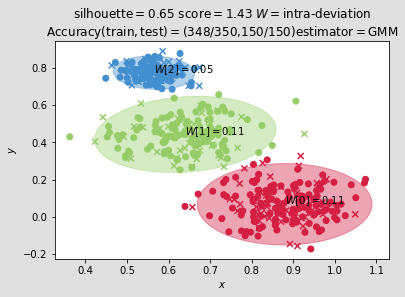
\includegraphics[width=0.23 \textwidth]
       {gmm_results/gmm_diff_sizes.png}
      }  
    \subfloat [Slender]
      {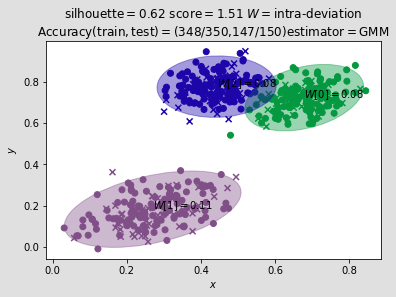
\includegraphics[width=0.23 \textwidth]
       {gmm_results/gmm_slender.png}
      }  
    \subfloat [Spherical]
      {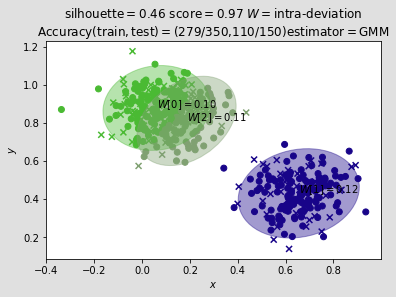
\includegraphics[width=0.23 \textwidth]
       {gmm_results/gmm_spherical.png}
      }  
    \subfloat 
    [ Populations 
     \footnote
       { $\#$points for each sub-cluster 
         $\mathcal{C}_{I}$ are distributed 
         by random weights.
       }
    ]
      {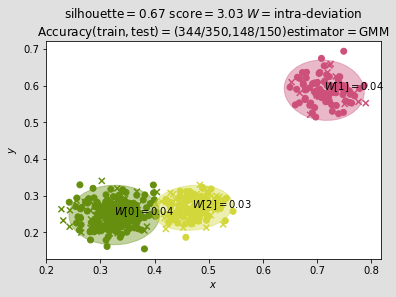
\includegraphics[width=0.23 \textwidth]
       {gmm_results/gmm_sparse.png}
      } 
  \end{figure} 
\item 2 cases where GMM fails to cluster correctly. 
  \begin{figure} [t!]
    \subfloat [Rings] 
      {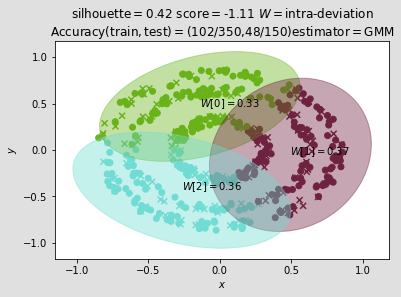
\includegraphics [width=0.23 \textwidth]
       {gmm_results/gmm_rings.png}
      }
    \subfloat [Blur] 
      {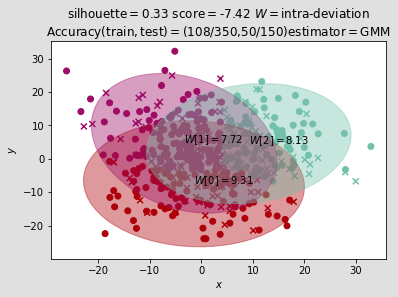
\includegraphics [width=0.23 \textwidth]
       {gmm_results/gmm_blur.png}
      }
  \end{figure} 
\end{itemize}
\end{frame} 

\begin{frame} [t] 
      {\bf Case Study: GMM continued}
\begin{itemize} 
\item Evaluating different scores on a parameter set of models 
      $\ksize \equiv \#\text{initial clusters}$.
  \begin{figure}
    \centering
    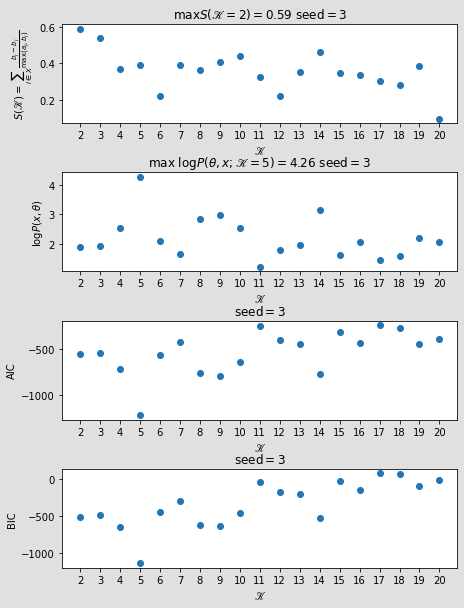
\includegraphics [width=0.30 \textwidth] 
    {gmm_results/gmm_compare_scores.png}
  \end{figure}
\item seed $\equiv \# \text{clusters used for data generation}$ 
\end{itemize}   
\end{frame}

\begin{frame} [t] {\bf Case Study: K-Means}
\begin{itemize}
\item K-means cluster different geometries of Gaussian blobs.
  \begin{figure}
    \centering
    \subfloat [Sizes]
      {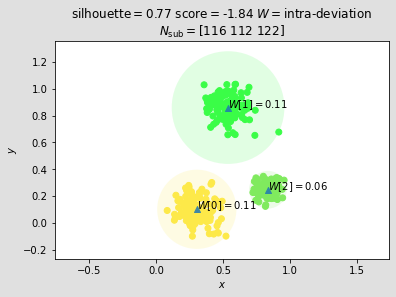
\includegraphics [width=0.23 \textwidth]
       {kmeans_results/diff_sizes_kmeans.png}
      }
    \subfloat [Identical]
      {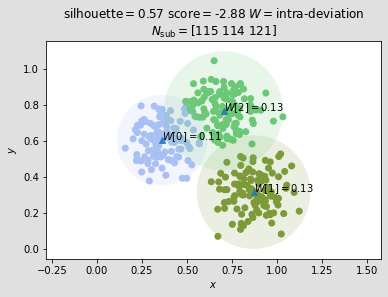
\includegraphics [width=0.23 \textwidth]
       {kmeans_results/identitical_blobs_kmeans .png}
      } 
    \subfloat [Slender]
      {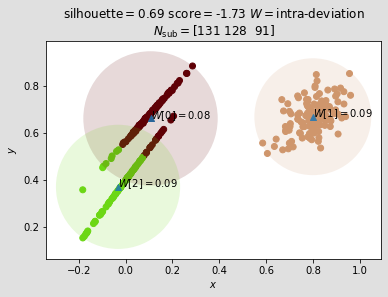
\includegraphics [width=0.23 \textwidth]
       {kmeans_results/slender_kmeans.png}
      } 
    \subfloat [Populations]
      {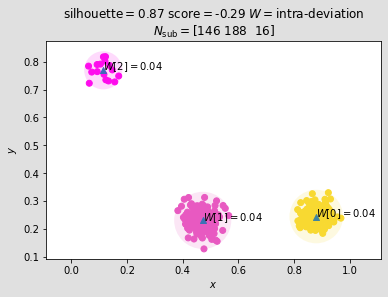
\includegraphics [width=0.23 \textwidth]
       {kmeans_results/sparse_kmeans.png}
      } 
  \end{figure}  
\item K-means failed to cluster rings (Gaussian error bars) 
      and blurry blobs.
  \begin{figure} 
    \centering
    \subfloat [Rings] 
      {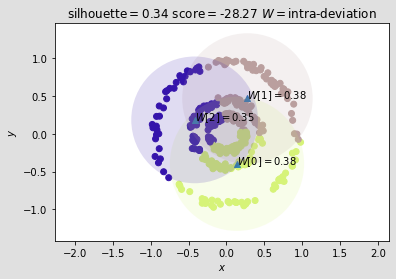
\includegraphics [width=0.23 \textwidth] 
       {kmeans_results/kmeans_rings}
      }
    \subfloat [Blur] 
      {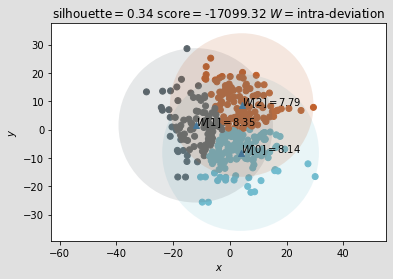
\includegraphics [width=0.23 \textwidth] 
       {kmeans_results/kmeans_blur}
      }
  \end{figure}
\end{itemize} 
\end{frame}

\end{document}